\chapter{Introduction}
\label{sec:intro}

In this document we outline the search for and characterization of the last undiscovered particle predicted by the Standard Model of Particle Physics. This model presents explanations for matter and energy in the universe. It has been tested and verified at the smallest distance scales and highest energies in the universe. To present the ideas outlined in this thesis, it is necessary to start with a collection of definitions. Some will be given here, while others are left to references or outside sources. 

\chaptermark{Introduction}

The natural starting point of this discussion is to present a useful example of symmetries that are observed in the world and how these are classified in physics. Next, a basic discussion of quantum field theory and scattering amplitudes will be presented. From these examples, the discussion will expand to a categorization of the particles, fields, and symmetries that make up the Standard Model of Particle Physics, including an introduction of Electroweak Symmetry Breaking. Equipped with these ideas an outline of Limitations of the Standard Model are presented using the Higgs boson as a tool for understanding them.

\section{Symmetries in Physics}
\label{sec:Symmetries}

Symmetry is one of, if not the, most important features in the physics of the natural world. As we pull together the various pieces needed to present the state of the art in particle physics, we will define multiple symmetries that exist in nature and how we use them to test our current and hypothetical models.

\subsection{Noether's Theorem}
\label{sec:Noether}

To begin, let us define the \textit{symmetry group} of the system, $G$, as the local group that transforms solutions into other solutions. If $x$ is a solution and $g$ is a group element, then $ g \cdot x$ will also be a solution. In Physics, the solutions that we consider either that maximize or minimize the action:  

\begin{equation}
\label{eq:action}
\mathcal{S} = \int d^{4}x{\mathscr{L}},
\end{equation}

where the integrand, $\mathscr{L}$, is the \textit{Lagrangian} of the system, $\mathscr{L} = T - V$. The $T$ and $V$ are the kinetic and potential energy, respectively. So a symmetry group of a physical system would be the set of transformations that leave the Lagrangian invariant. This concept became one of most important in physics after Emmy Noether proved that these symmetries of the action correspond to conserved quantities that do not change as the system evolves \cite{Noether:1918zz}.

\subsection{Angular Momentum and the Rotation Group}
\label{sec:AngularMomentum}

To demonstrate the importance of Noether's Theorem, let us consider the group of rotations in 3 dimensional space, the special orthogonal group in 3 dimensions, $\mathrm{SO}(3)$. Given any unit vector $\hat{\textbf{n}}$ a rotation about this vector by an angle $\psi$ is denoted by $R_{\hat{\textbf{n}}}(\psi)$. Here we will use the Euler Angles to parameterize $R$, where the rotations about the $(x,y,z)$ axis are given by $(\alpha, \beta, \gamma)$ respectively. It will also be useful to note that performing a rotation $R_{1}$ followed by another rotation $R_{2}$ is equivalent to a single rotation $R_{3}$, or that the set of rotations is closed.

\begin{figure}
\begin{center}
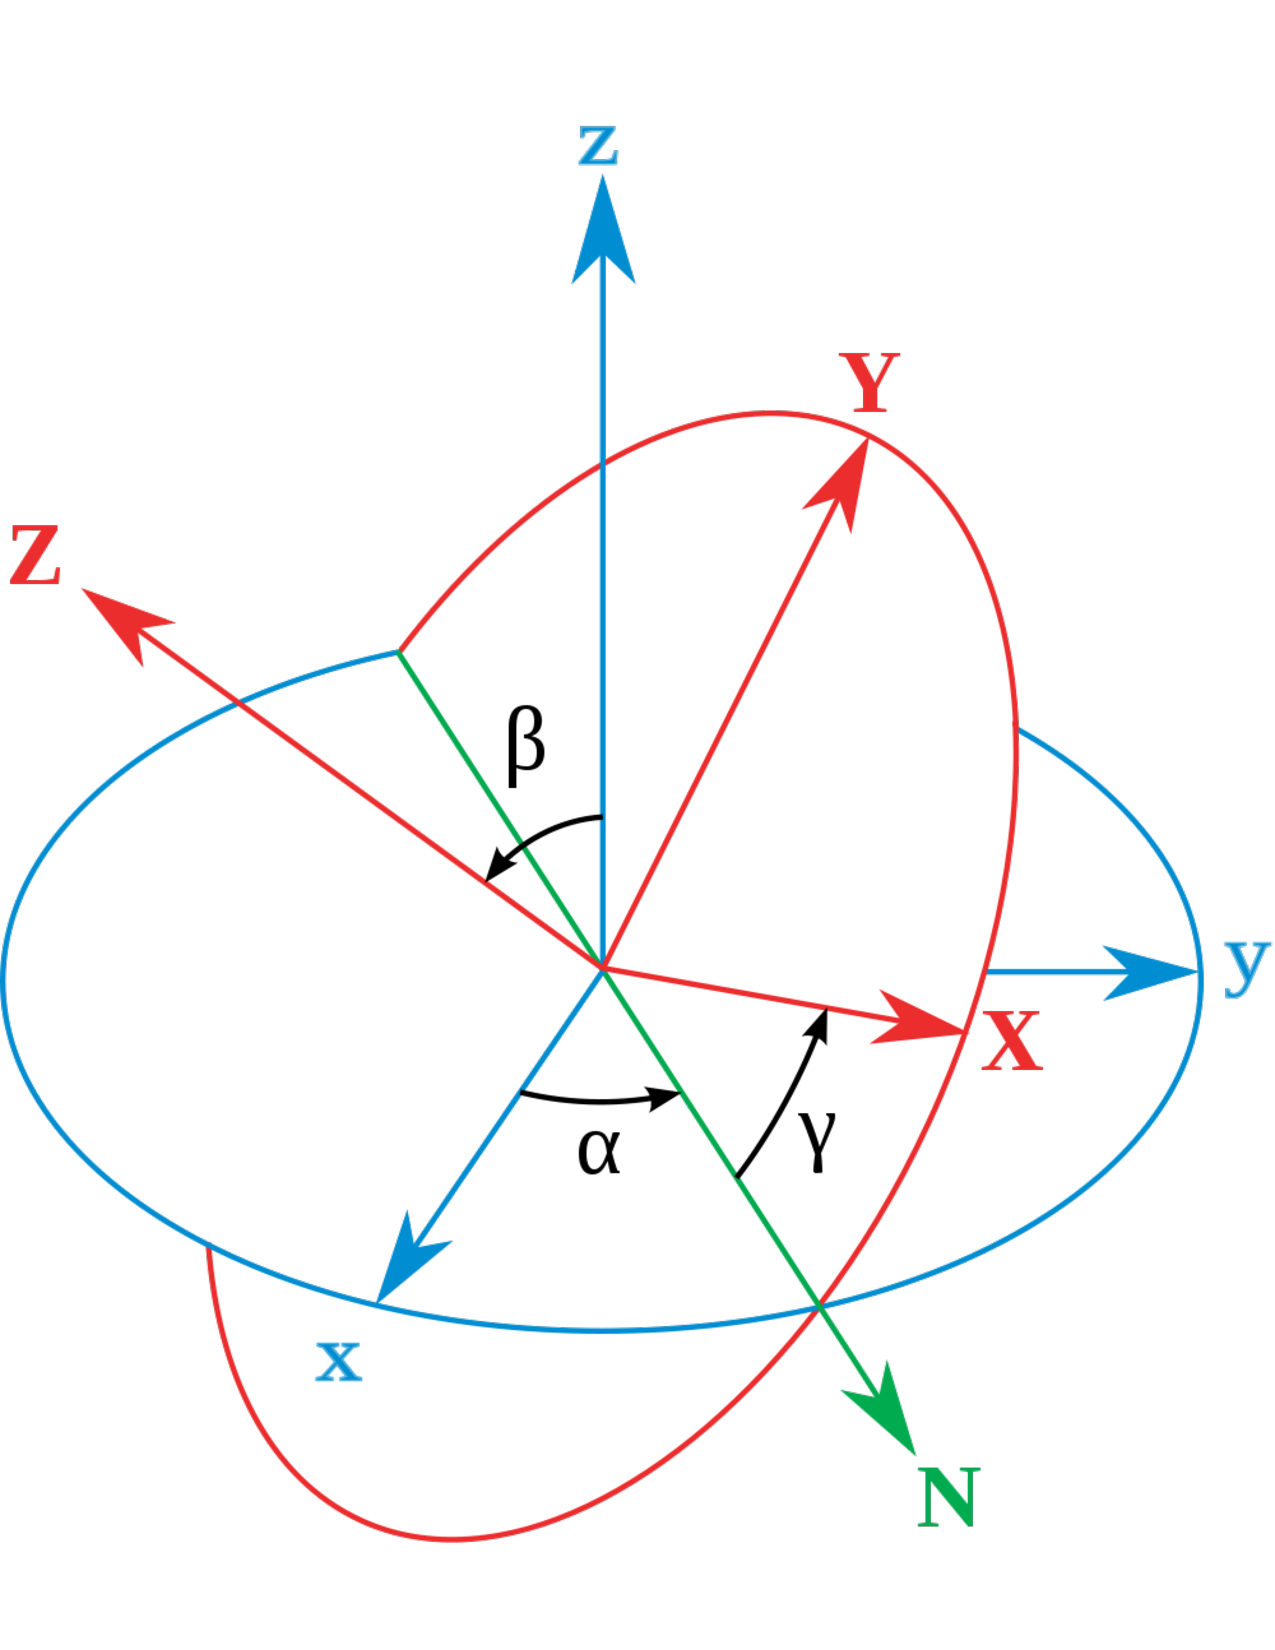
\includegraphics[width=0.35\linewidth]{Introduction/Euler.pdf}
\caption[Euler angles for three dimensional Cartesian coordinates.]{Euler angles for three dimensional Cartesian coordinates.\cite{wiki:Euler}}
\label{fig:Euler}
\end{center}
\end{figure}


A arbitrary rotation $R(\alpha, \beta, \gamma)$ can be decomposed into rotations about the fixed axes, $R(\alpha, \beta, \gamma) = R_{x}(\alpha)R_{y}(\beta)R_{z}(\gamma)$. Figure \ref{fig:Euler} shows these angles for the transformation of vector $N$ from $(x,y,z)$ to $(X,Y,Z)$. At this point it is useful to express the rotations $R_{x,y,z}$ in terms of their matrix formulation, equations \eqref{eq:Second}, \eqref{eq:Third}, \eqref{eq:Fourth}. Where the angle of rotation must satisfy $0 \leq \psi \leq 2\pi$.

\begin{equation}
\label{eq:Second}
R_{z}(\gamma) = \left( \begin{array}{ccc}
\cos\gamma & -\sin\gamma & 0 \\
\sin\gamma & \cos\gamma & 0 \\
0 & 0 & 1 \end{array} \right)
\end{equation}

\begin{equation}
\label{eq:Third}
R_{y}(\beta) = \left( \begin{array}{ccc}
\cos\beta & 0 & \sin\beta \\
0 & 1 & 0 \\
-\sin\beta & 0 & \cos\beta \end{array} \right)
\end{equation}

\begin{equation}
\label{eq:Fourth}
R_{x}(\alpha) = \left( \begin{array}{ccc}
1 & 0 & 0 \\
0 & \cos\alpha & -\sin\alpha \\
0 & \sin\alpha & \cos\alpha \end{array} \right) 
\end{equation}

The reader should note that a vector along the $z$-axis direction will be left unchanged due to a $R_{z}$ rotation. More generally, we can apply Noether's Theorem when the Lagrangian for a physical system does not depend on infinitesimal rotations about any axis, $\mathscr{L}-\mathscr{L}(\delta\alpha,\delta\beta,\delta\gamma) = 0$. This symmetry corresponds to the classical conservation of angular momentum, $\mathrm{J}$, when the Lagrangian has spherical symmetry. This symmetry will become important as we discuss the kinematics of the particles we use to study new discoveries.

\subsection{Inherent Spin and $\mathrm{SU}(2)$}
\label{sec:SU2}

If one fixes a direction in equations \eqref{eq:Second}, \eqref{eq:Third}, and \eqref{eq:Fourth} then the rotations about that direction will form a subgroup of $\mathrm{SO}(3)$. This becomes clear when you consider the closure, identity, and inverse group axioms for the subset of rotations $R_{z}$. Specifically, the subgroup is isomorphic to the special unitary group of rotations in two dimensions, $\mathrm{SU}(2)$. One way to write this new transformation is: 

\begin{equation}
\label{eq:Dim2}
R(\phi) = \left( \begin{array}{cc}
\cos\phi & -\sin\phi \\
\sin\phi & \cos\phi \end{array} \right)
\end{equation}

The simplest way to represent a group is to find the elements that all other elements of the group can be made from. To find these elements for $\mathrm{SU}(2)$ start with equation \eqref{eq:Dim2} and consider an infinitesimal rotation $d\phi$. Since $R(\phi)$ is differentiable one can derive an equation to write all possible rotations in terms of the operator matrix $\mathrm{J}$ which we will call the \textit{generator} of $\mathrm{SU}(2)$. Explicitly, $R(\phi)$ can be written as:

\begin{equation}
\label{eq:generator}
R(\phi) = e^{-i \frac{\phi}{2} \mathrm{J}},
\end{equation}

where $\mathrm{J}_{i} = \tau_{i}$ and $\tau_{i}$ is one of the Pauli matrices:

\begin{equation}
\label{eq:Pauli}
\tau_{1} = \begin{pmatrix}
    0 & 1\\
    1 & 0
  \end{pmatrix}, \tau_{2} = \begin{pmatrix}
    0 & -i\\
    i & 0
  \end{pmatrix}, \tau_{3} = \begin{pmatrix}
    1 & 0\\
    0 & -1
  \end{pmatrix}
  \end{equation}


In this formulation $R(\phi)$ operates on states that are linear combinations of \textit{two-component spinors} given by equation \eqref{eq:spinors}. These spinor eigenstates have an inherent conserved spin of $\pm\hbar/2$. 

\begin{equation}
\label{eq:spinors}
\chi_{+} = \begin{pmatrix} 1 \\ 0 \end{pmatrix}, \chi_{-} = \begin{pmatrix} 0\\1\end{pmatrix}
\end{equation}

These states can be expressed as linear combinations of these two component spinors, but we will find it more useful to transform the basis so that they can be rewritten in terms of the two component spinors $\psi_{R}$ (right-handed) and $\psi_{L}$ (left-handed) that are eigenstates of the parity transformation\footnote{As position transforms from $\vec{x} \to -\vec{x}$ the momentum transforms as $\vec{p} \to -\vec{p}$}.

\begin{equation}
\label{eq:TwoRandL}
\psi = \begin{pmatrix} \psi_{R} \\ \psi_{L} \end{pmatrix}
\end{equation}

These states, called \textit{fermions}, and the group $\mathrm{SU}(2)$ will be two of the major building blocks that are used when we discuss the Standard Model of particle physics. Before we describe this model we will take some time to discuss Scattering Amplitudes.

\section{Scattering Amplitudes}
\label{sec:Scattering}

Particle physics research at its core is not very different from pre-school; we want to see what is inside of something but can't get our hands in the tiny spaces, so we smash it apart. The complexity that is swept under the rug in this statement is that we can map what is happening in these small spaces to what we observe using scattering amplitudes, which tell us the behavior of particles as they "break away" from the things we are trying to study. More generally, a scattering matrix tells us how a system of particles will evolve over time, either because of collisions between particles or other natural processes.

\subsection{Scattering Matrix}
\label{sec:Smatrix}

To explain how particle physics explains the evolution of a system over time, we will follow a procedure outlined in \cite{Maggiore5.1:2005}. Let us consider a set of particle fields with certain characteristics denoted $\ket{\psi}\left(t\right)$. The system at a time $t$ is given in Dirac notation\cite{Schwabl:2002}. We will denote the initial state of the system as $\ket{\psi_{i}} = \ket{\psi}\left(t_{i}\right)$, and the final state as $\ket{\psi_{f}} = \ket{\phi}\left(t_{f}\right)$. These states can be single or multiple particle states and typically quantities like momentum, spin, or helicity\footnote{Projection of spin onto momentum, $\vec{S}\cdot\hat{p}$} are used to specify them in this notation.

The evolution of a system from state $\ket{\psi_{i}}$ to $\bra{\psi_{f}}$ is given by
\begin{equation}
\label{eq:psiSpsi}
\bra{\psi_{f}}S\ket{\psi_{i}},
\end{equation}
where $S$ is a quantum mechanical operator associated with the scattering matrix. 

To give a concrete example you can consider a plane wave evolving over time. In this case, $S = e^{-iH\left(t-t_{i}\right)}$. For this explanation, we use a Hamiltonian $H$ instead of a Lagrangian, but a Hamiltonian is simply the Legendre transformation of a Lagrangian, so they are equivalent for our purpose. In this case, equation \eqref{eq:psiSpsi} becomes

\begin{equation}
\label{eq:WaveSmatrix}
\bra{\psi_{f}}e^{-iH\left(t_{f}-t_{i}\right)}\ket{\psi_{i}}.
\end{equation}

In the limit that $t_{f} - t_{i} \to \infty$ the operator between the states is the \textit{scattering matrix} and maps some initial state to a final state at some other time. 

\subsection{Amplitudes and Feynman Diagrams}
\label{sec:Amplitudes}

Each of the states outlined in the previous section, $\ket{\psi}\left(t\right)$, will have specific properties. For example, the initial state may be in eigenstate $a$ for some commuting operator, while the final state may be in eigenstate $b$ of the same operator. Then the evolution of the system from $\ket{a}$ to $\ket{b}$ will be through a specific \textit{matrix element}, $\mathcal{M}_{ab}$.

\begin{equation}
\label{eq:bSa}
\mathcal{M}_{ab} = \bra{b}S\ket{a}
\end{equation}

These matrix elements can be used to describe the evolution of the system through very specific transitions. These matrix elements are also called \textit{scattering amplitudes}, $\mathrm{A}$, for a specific process.
\begin{equation}
\label{eq:Amplitude}
\mathrm{A}_{ab} = \mathcal{M}_{ab} = \bra{b}S\ket{a}
\end{equation}

These amplitudes can also be expressed in a pictorial form, called \textit{Feynman diagrams}, that we will use extensively in this document. These diagrams are used to do the calculations through rules mapping vertex points, internal, and external lines to terms in the matrix element pieces.


To use a concrete example, we will describe the interaction of electrons through the electromagnetic interaction. The Lagrangian for two fermions interacting elecgromagneticily is given by 
\begin{equation}
\label{eq:EMlagrangian}
\mathscr{L}_{EM} = \bar{\psi} \left(i\gamma^{\mu}\left(\partial_{\mu} + ieA_{\mu}\right) - m\right)\psi.
\end{equation}

In this equation, the electromagnetic interaction terms are represented by the vector potential, $A_{\mu}$, with $e$ as the coupling constant of the particle to the electromagnetic field. The $4 \times 4$ Dirac matrices $\gamma^{\mu}$ are defined by the $2 \times 2$ Identity matrix $\left(1\right)$ and the Pauli-matrices we have already seen

\begin{equation}
\label{eq:GammaMatrix}
\gamma^{0} = \begin{pmatrix} 1 & 0 \\
					       0 & -1 \end{pmatrix},
\gamma^{i} = \begin{pmatrix} 0 & \tau^{i} \\
                                               -\tau^{i} & 0 \end{pmatrix}.
\end{equation}

In the amplitude notation this can be written as
\begin{equation}
\label{eq:eeScatteringAmpl}
A = \bra{\psi_{1}\psi_{2}}e^{\bar{\psi}\left(i\gamma^{\mu}\left(\partial_{\mu} + ieA_{\mu}\right) - m\right)\psi}\ket{\psi_{1}\psi_{2}}
\end{equation}

The equivalent representation lowest order terms of equation \eqref{eq:EMlagrangian} as Feynman diagrams will be figure \ref{fig:eeScattering}. These diagrams can be used to quickly and simply represent complex interactions of particles and range from very simple, figure\ref{fig:eeScattering}, to extremely complex, as in the comedic example \ref{fig:Jayhawk_Feynman}. Relevant and practical examples will be presented in section \ref{sec:LHC_Pheno}.

\begin{figure}
\begin{center}
\unitlength=1mm
\begin{fmffile}{eeScattering}

\begin{fmfgraph*}(40,30) \fmfpen{thick}
  \fmfleft{i1,i2} \fmfright{sp1,sp2}
  \fmf{fermion,label=$e^-$}{i1,v1,sp1} 
  \fmf{fermion,label=$e^-$}{i2,v2,sp2}
  \fmf{photon,label=$\gamma$}{v1,v2}
\end{fmfgraph*}

\end{fmffile}
\end{center}
\caption[Feynman diagram depicting electron-electron scattering via the electromagnetic interaction.]{Feynman diagram depicting electron-electron scattering via the electromagnetic interaction.}
\label{fig:eeScattering}
\end{figure}

\begin{figure}
\begin{center}
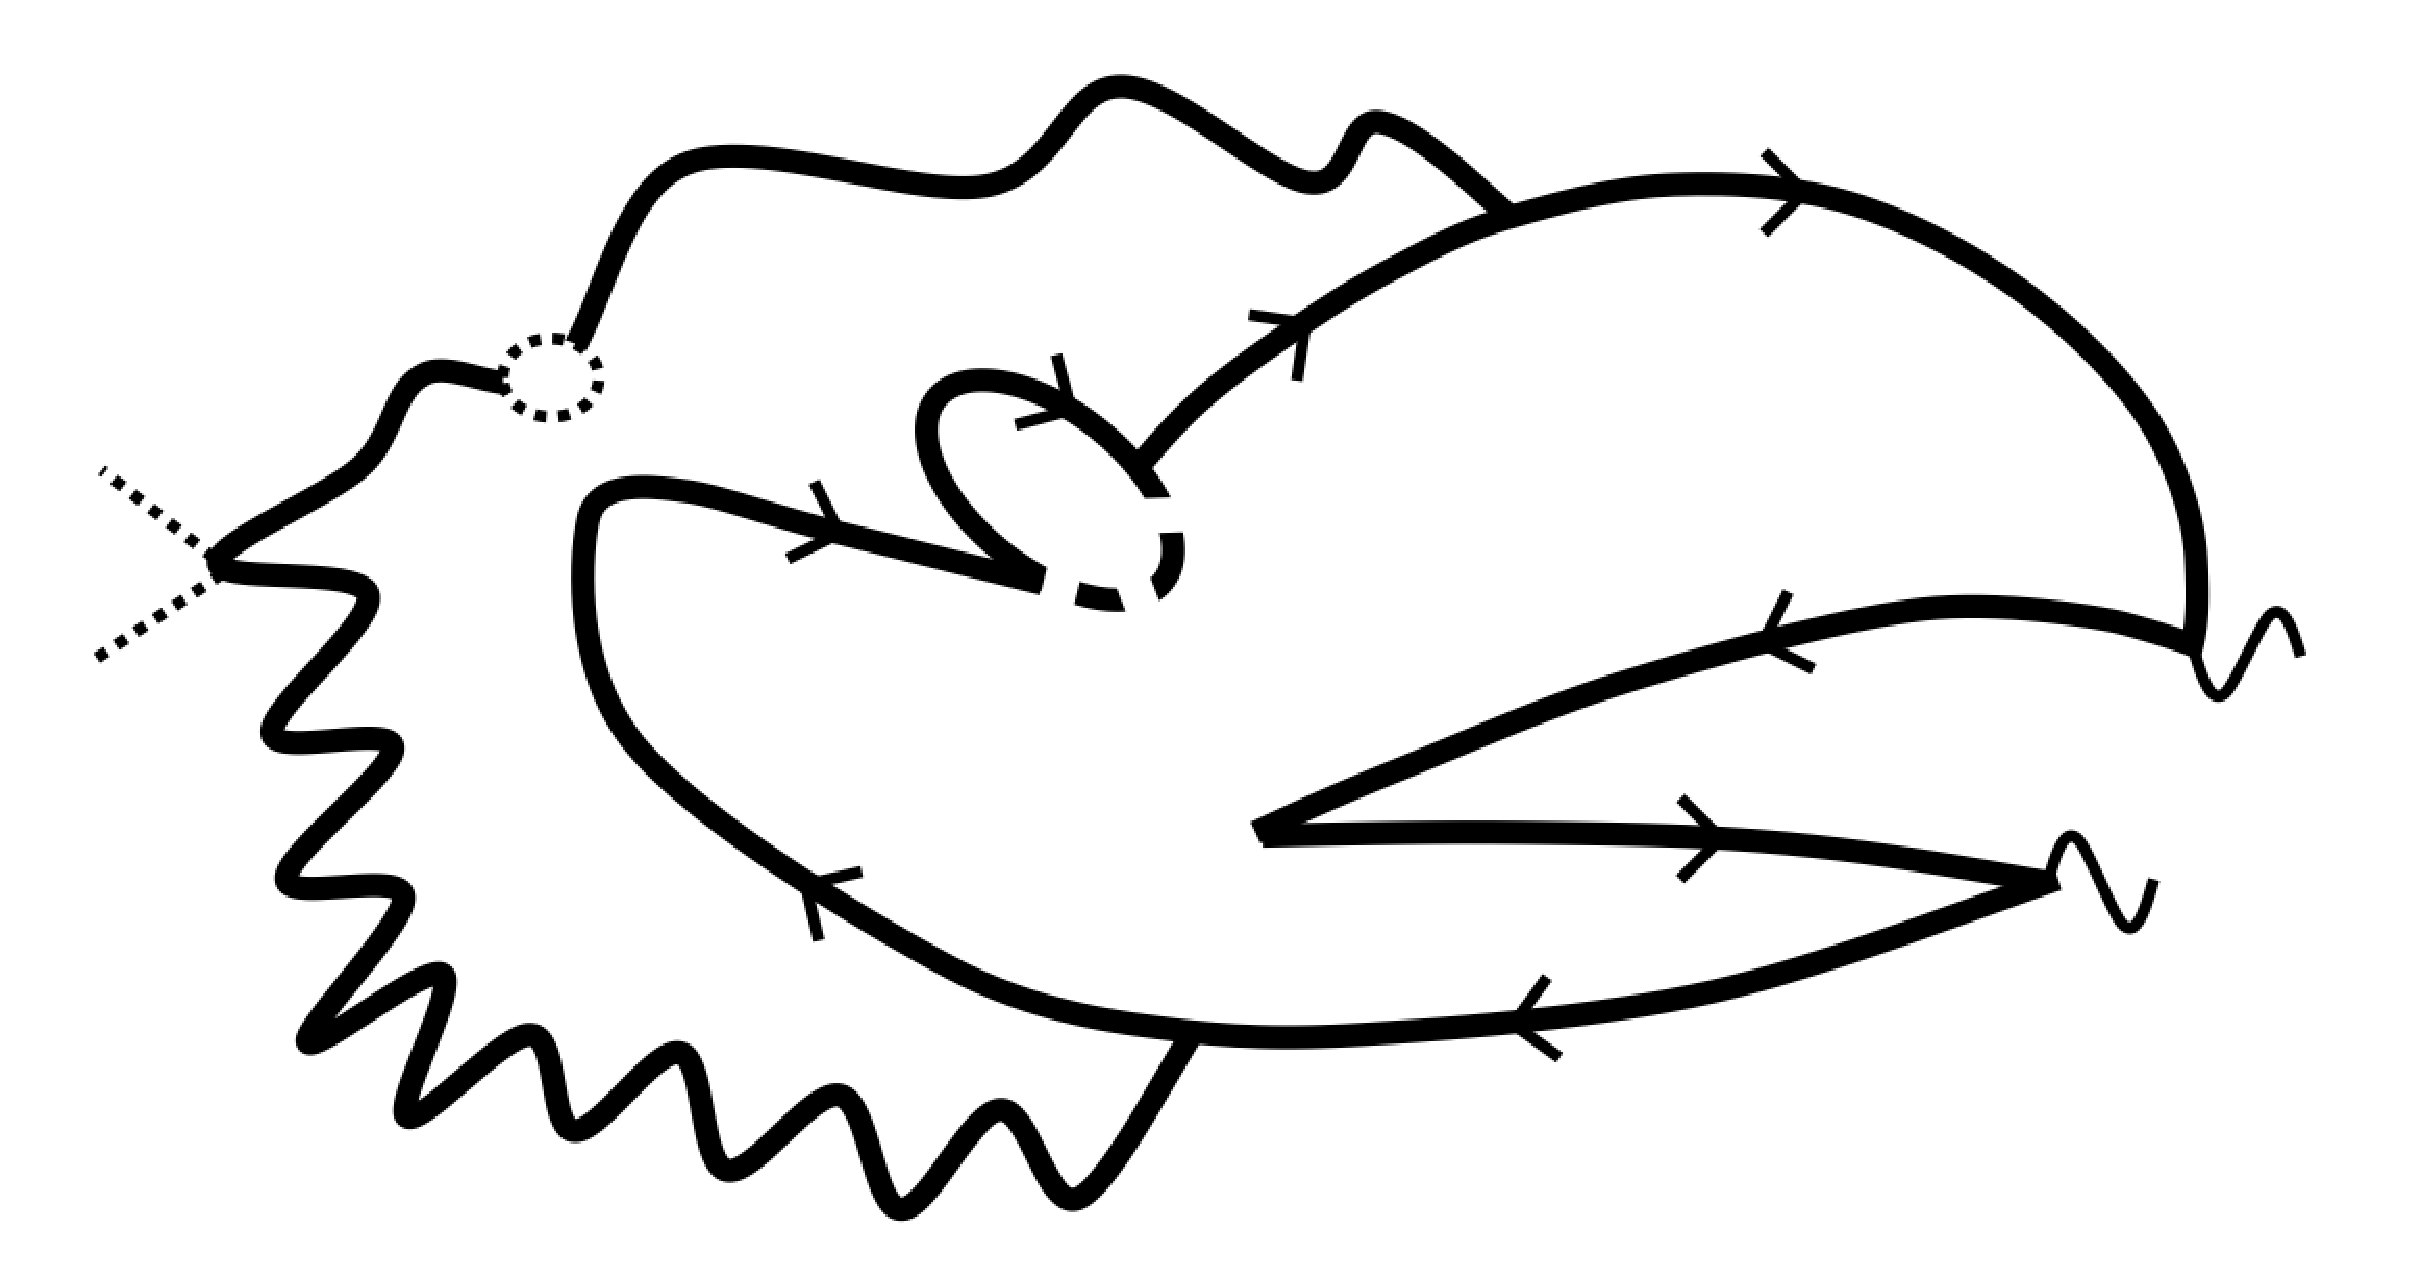
\includegraphics[width=0.5\linewidth]{Introduction/Jayhawk_Feynman.pdf}
\caption[A comedic example of a complicated Feynman diagram designed to appear similar to a Jayhawk.]{A comedic example of a complicated Feynman diagram designed to appear similar to a Jayhawk \cite{Hogan:2007jh}.}
\label{fig:Jayhawk_Feynman}
\end{center}
\end{figure}

In this example we can see the properties of another group that will be important for the Standard Model. The electromagnetic interaction requires $\mathrm{U}(1)$ gauge symmetry. The conserved quantity for this group is the electric charge of the fermion, given by $e$ in the equations above. Now that we have introduced many of the pieces we need we will discuss the Standard Model of particle physics.

\section{The Standard Model}
\label{sec:TheSM}
So far we have considered very simple Lagrangians that describe very specific processes. These ideas are the basis for the construction of the \textit{Standard Model} (SM) \cite{StandardModel67_1,StandardModel67_2,StandardModel67_3,StandardModel67_4} of particle physics. This model attempts to describe and categorize the particles and interactions that make up the quantum world. The glaring omission is gravity, which is extremely weak compared to the other processes that are occurring at sub-atomic distance scales. Before we can discuss how the model describes the fundamental interactions we need to describe and categorize the material that the universe is made from.

\begin{figure}
\begin{center}
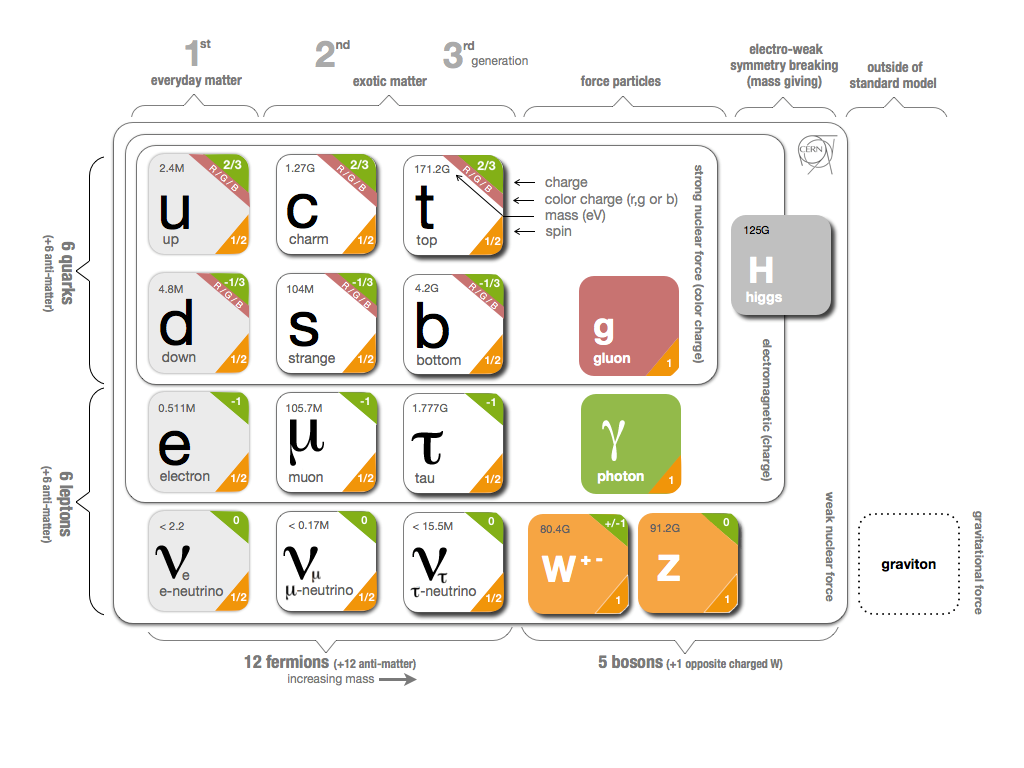
\includegraphics[width=\linewidth]{Introduction/SMinfographic_image.png}
\caption[A Summary Infographic of The Standard Model.]{A Summary Infographic of the Standard Model. This is a modified version of original found at \cite{SMinfo:2012sm}.}
\label{fig:TheSM}
\end{center}
\end{figure}

\subsection{Matter}
\label{sec:TheMatter}

The SM provides a categorization of all the matter that makes up the universe. This categorization started with the first experiments attempting to describe atoms distinguishing the particles in the nucleus of an atom from the electrons that orbit around them. Today we know of matter in two categories, \textit{quarks} and \textit{leptons}, both of which are fermions with spins of $\hbar/2$, noted $1/2$ from now on\footnote{Here we have moved to the convention of natural units where $\hbar = c = 1$}. For each of these categories there are three generations of particles, each generation consisting of two quarks ($q$), two leptons ($\ell$) and their antiparticles\footnote{The antiparticle of a fermion is the $C$ transform of the particle state. $C$ transforms discussed more in section \ref{sec:CPviolation}}($\bar{q}, \bar{\ell}$). The heavier second and third generation fermions typically decay quickly into the first generation particles that make up the world we live in\footnote{The neutrino's being the exception to this.}.

\subsubsection{Quarks}
\label{sec:TheQuarks}

Quarks are the fundamental pieces that make up the nucleus of atoms. The protons and neutrons that are used to classify an atom are themselves built form combinations of quarks. The name ``quark" was coined by Gell-Mann who credits the term to a passage from \textit{Finnegans Wake} by James Joyce. Quarks come in six \textit{flavors} arranged by mass into three generations of doublets, this flavor is preserved in electromagnetic and strong interactions. The first letter of the quark name is often used to designate them so up $\left(u\right)$, down $\left(d\right)$, charm $\left(c\right)$, strange $\left(s\right)$, top $\left(t\right)$, and bottom $\left(b\right)$. Each flavor has a different mass ranging from $\sim\unit{}{\MeV}$ ($u$ and $d$) to $\sim\unit{170}{\GeV}$ $\left(t\right)$, the best knowledge of these masses is outlined in figure \ref{fig:TheSM}.

Everyday matter consists mainly of the first generation quarks, u and d, grouped into the protons and neutrons. Quarks are never observed alone due to a \textit{color charge} that each posses\footnote{The property has nothing to do with optical color, but maps nicely to the mixing fundamental colors.}. This will be discussed more in section \ref{sec:TheForces}, but for now we will refer to it as a charge that can be ``red" (\textcolor{myred}{r}), ``blue" (\textcolor{myblue}{b}), or ``green"(\textcolor{mygreen}{g}). To be stable, a particle must be seen as  ``white" (\contour{black}{\textcolor{white}{w}}) to the outside world. Because matter must appear white, quarks group themselves into sets called \textit{hadrons}. Hadrons come in classifications based on the number of valence quarks they have. Two quark states are quark-antiquark pairs called \textit{mesons}, $\left(\textrm{\textcolor{myred}{r}}\textcolor{myred}{\bar{\textrm{r}}} + \textrm{\textcolor{myblue}{b}}\textcolor{myblue}{\bar{\textrm{b}}} + \textrm{\textcolor{mygreen}{g}}\textcolor{mygreen}{\bar{\textrm{g}}}\right)/\sqrt{3} = \textrm{\contour{black}{\textcolor{white}{w}}}$. Common examples of mesons are pions $\left(\pi^{0},\pi^{\pm}\right)$ that come from cosmic rays. Three quark states are called \textit{baryons}, $\mathrm{\textcolor{myred}{r}} + \mathrm{\textcolor{myblue}{b}} + \mathrm{\textcolor{mygreen}{g}} = \mathrm{\contour{black}{\textcolor{white}{w}}}$, everyday examples being protons and neutrons. Recent observations also suggest tetraquark states \cite{Aaij:2014jqa} consisting of four quarks. 

Each quark generation doublet has one particle with electromagnetic charge\footnote{``$e$" is used as the fundamental unit of electromagnetic charge. ``$-e$" is defined as the charge of an electron.} of $+2/3 e$ and another with charge $-1/3 e$. These will be combined so that all observable hadrons will have integer charges. The top-left section of figure \ref{fig:TheSM} summarizes the properties and categorization of the quarks. 

One additional item that will prove relevant is that quarks can be both right-handed and left-handed eigenstates of the parity transform. This will distinguish their interactions when we discuss the weak force in section \ref{sec:TheForces}.

\subsubsection{Leptons}
\label{sec:TheLeptons}

Unlike the quarks, leptons cary no property that stops them from existing by themselves. All leptons are neutral to color charge preventing them from interacting via the strong nuclear force. The most common lepton again belongs to the first generation, the electron. Electrons orbiting the nucleus of an atom are the most common leptons. Similar to the heavier generations of the quarks, the electron also has corresponding heavier generation flavors, the muon ($\mu$) and tau ($\tau$) leptons. All three of these leptons cary an electromagnetic charge of ``$-e$", range in mass from $\sim\unit{0.5}{\MeV}$($e$) to $\sim\unit{1.7}{\GeV}$($\tau$), and can exist both as left or right-handed.

Each of these three leptons has a corresponding doublet parter as well, the neutrinos ($\nu_{e}, \nu_{\mu}, \nu_{\tau}$). These particles are neutral in both color and electromagnetic charge, and are almost massless. Further complicating the story, they only exist as left-handed particles. They are extremely hard to interact with and detect since the electromagnetic and strong forces are invisible to them allowing them to only interact via the weak nuclear force. Additionally, unlike the quarks and the other leptons, they oscillate between different flavors without interacting with the environment because their mass eigenstates are not the same as their weak interaction eigenstates. In \ref{fig:TheSM} the leptons occupy the bottom left portion of the table. A summary of the first generation fermion fields that are given in table \ref{tab:FermionFields} where the doublets are grouped together and the distinction between left and right-handed particles has been made.

\begin{table}
\begin{center}
\begin{tabular}{c|c|c|c||c}
\hline 
\hline
Fermion Field & EM charge $\left(Q\right)$ & Weak Isospin $\left(T_{3}\right)$ & Hyperchage $\left(Y\right)$ & Color Charge \\ \hline
$L_{L} = \begin{pmatrix} \nu_{L} \\ e^{-}_{L} \end{pmatrix}$ & $\begin{pmatrix} 0 \\ -1 \end{pmatrix}$ & $\begin{pmatrix} +1/2 \\ -1/2 \end{pmatrix}$ & $-1$ & no \\
$e_{R}^{-}$ & $-1$ & $0$ & $-2$ & no \\
\hline
$Q_{L} = \begin{pmatrix} u_{L} \\ d_{L} \end{pmatrix}$ & $\begin{pmatrix} +2/3 \\ -1/3 \end{pmatrix}$ & $\begin{pmatrix} +1/2 \\ -1/2 \end{pmatrix}$ & $+1/3$ & yes \\
$u_{R}$ & $+2/3$ & $0$ & $+4/3$ & yes \\
$d_{R}$ & $-1/3$ & $0$ & $-2/3$ & yes \\
\hline
\hline
\end{tabular}
\end{center}
\caption[First generation fermions and their different charges, grouped in left(right)-handed doublets(singlets).]{First generation fermions and their different charges, grouped in left(right)-handed doublets(singlets).}
\label{tab:FermionFields}
\end{table}


While the only leptons in everyday matter are electrons, muons and neutrinos are also quite common. These particles exist as cosmic rays that are constantly bombarding us from the upper atmosphere and outer space. Muons offer a particularly interesting case because they are moving at relativistic speeds so that in our frame of reference they appear as long lived particles.

\subsection{Forces}
\label{sec:TheForces}

Now that we have introduced the building blocks of matter we can discuss how these particles interact. This description starts with a Lagrangian of terms describing particles and their interactions with each other, however this Lagrangian needs to preserve specific symmetries that we observe in nature. Specifically the SM Lagrangian should have $\mathrm{U}(1) \times \mathrm{SU}(2) \times \mathrm{SU}(3)$ local symmetry\footnote{The difference between a local and global symmetry has not been outlined in this document, but the author again refers you to \cite{Armstrong:1988,Miller:1972,Oliver:1993,Tung:1985} and many other places.}. Each of these symmetries correspond to physical interactions between the particles in the theory. Mathematically it is extremely similar to equation \eqref{eq:EMlagrangian}, however the $\left(\partial_{\mu} + ieA_{\mu}\right)$ is replaced by the more complicated covariant derivative $\mathcal{D}_{\mu}$.

\begin{equation}
\label{eq:CovariantD}
\mathcal{D}_{\mu} = \partial_{\mu} - i g_{1} \frac{\mathrm{Y}}{2}B_{\mu} - i g_{2} \frac{\tau^{i}}{2}W^{i}_{\mu} - i g_{3} \frac{\lambda^{a}}{2}G^{a}_{\mu}
\end{equation}

Each of these additional terms are present to preserve one of the local symmetries that we observe in the world. Each of the $g_{i}$ variables are coupling constants that can be measured by experimental results. These new fields map to the fundamental forces and in turn \textit{gauge bosons} that mediate each of the forces. They are called bosons because they have an integer unit of inherent spin, as apposed to the matter particles that all have half-integer spin. Particle physics models fermions interacting with each other as the exchange of these bosons between particles.

A rather glaring omission from both equation \eqref{eq:EMlagrangian} and the extension using equation \eqref{eq:CovariantD} is how these new fields (bosons) interact with themselves and each other. We will not take the time to introduce all of these terms but the relevant pieces will be used in section \ref{sec:EWsymmetry}.

The term associated with $g_{1}$ is introduced to preserve local gauge invariance, $\mathrm{U}(1)$, introducing a spin-1 field $B_{\mu}$. The generator, $\mathrm{Y}$ (\textit{hypercharge}), will be a constant for every particle. This term, intertwined with the $g_{2}$ term, describes the \textit{electromagnetic force}. The $g_{2}$ term, along with the $g_{1}$ term, describes the \textit{weak nuclear force}. The details of their combination will be described in section \ref{sec:EWsymmetry}. 

The $g_{2}$ term preserves rotations in flavor space, $\mathrm{SU}(2)$, introducing three new vector fields $W^{i}_{\mu}$ where $i \in \left\{1, 2, 3\right\}$ and the generators $\tau^{i}$ (the Pauli matrices we have already seen). Similar to the case of angular momentum we have already seen, the $i=3$ projection, $T_{3}$, is a conserved quantity called \textit{weak isospin} that is useful in computations.

Additionally, the $W^{i}_{\mu}$ bosons are exclusively left-handed, meaning it can only interact with left-handed particles (right-handed antiparticles). For now, it is useful to note that both the $B_{\mu}$ and the $W^{3}_{\mu}$ terms represent interactions that preserve the original flavor of the fermions they act on. In the framework of equation \eqref{eq:EMlagrangian} and figure \ref{fig:eeScattering} this means that the photon field, $A_{\mu}$, is some linear combination of $B_{\mu}$ and $W^{3}_{\mu}$ and the electroweak charge, $e$, is a linear combination of $g_{1} \frac{\mathrm{Y}}{2}$ and $g_{2} \frac{\tau^{3}}{2}$.

The final term associated with $g_{3}$ represents the \textit{strong nuclear force} and preserves rotations in the color charge space, $\mathrm{SU}(3)$. This term introduces eight new vector fields $G^{a}_{\mu}$ with $a \in \left\{1, 2, 3, 4, 5, 6, 7, 8\right\}$ and eight generators $\lambda^{a}$ which are the analog of the Pauli matrices in 3 dimensions. Each of these fields corresponds to a \textit{gluon} that mediates the strong force. These interactions are described by Quantum Chromodynamics (QCD), the quantum field theory for how particles with color charge (quarks \& gluons) interact with each other. The conserved charge in this theory is the color; ``redness", ``blueness", and ``greenness". Each of the eight gluons in this theory is a superposition of color charge states and ``holds" quarks of specific colors together into colorless hadrons. An explicit listing of the gluon states is not provided here, but a basic introduction can be found in \cite{Griffiths9:1987tj}.

Before going through the details of the electromagnetic and weak forces, a quick note on the relative strength of these interactions. The electromagnetic force is common in every day life because it is a relatively strong interaction and operates over long distances, for example the light from a distant star can be seen at night. The strongest of the forces is the strong nuclear force which keeps the quarks grouped in hadrons and hadrons together in a nucleus is much stronger but only impacts particles that are very close together. At larger distances the weakest of the forces considered in particle physics is the creatively named weak nuclear force, which governs the decay of higher generation fermions into lower generation fermions. In table \ref{tab:Forces} you can find a summary of the different forces and their relative strengths and interaction ranges.

Included in this table is the gravitational force. There are theoretical models for describing quantum gravity in the same framework as these other forces, that will be discussed more in later sections but as yet these have not been confirmed with observations.

\begin{table}
\begin{center}
\begin{tabular}{c|c|c|c}
\hline 
\hline
Force & Bosons & Relative Strength & Range (m) \\ \hline \hline
Strong & gluons $\left(g\right)$ & 1 & $10^{-15}$ \\
Electromagnetic & photon $\left(\gamma\right)$ & $\frac{1}{137}$ & $\infty$ \\
Weak & $W^{\pm}, Z$ bosons & $10^{-6}$ & $10^{-18}$ \\
Gravity & graviton $\left(G\right)$ & $10^{-39}$ & $\infty$ \\
\hline
\end{tabular}
\end{center}
\caption[List of Fundamental Forces their relative strengths and ranges.]{List of Fundamental Forces their relative strengths and ranges.}
\label{tab:Forces}
\end{table}

\subsection{Electroweak Symmetry Breaking}
\label{sec:EWsymmetry}
As eluded to above, the weak and electromagnetic forces are deeply connected. In their combined form they are referred to as the \textit{Electroweak force}. In the description we outlined, this means that the SM has $\mathrm{SU}(2) \times \mathrm{U}(1)$ symmetry, giving rise to four gauge bosons that would mediate these two forces; $B_{\mu}$, $W_{\mu}^{1}$, $W_{\mu}^{2}$, and $W_{\mu}^{3}$. In the mathematical construction that we have presented all of these $W_{\mu}^{i}$ bosons would be massless, but this would contradict the observed range of the weak force outlined in Table \ref{tab:Forces}. To give these bosons mass, the symmetry of the system must be broken. The \textit{Higgs Mechanism} \cite{Higgs:1964ia,Higgs:1964pj,Higgs:1966ev,Englert:1964et,Guralnik:1964eu,Kibble:1967sv} has been proposed as the source of the \textit{Electroweak Symmetry Breaking} \cite{Dawson:2008jk}. 

To see how this happens, focus on the kinetic energy terms of the $W_{\mu}^{i}$ and $B_{\mu}$ fields that we neglected previously. These are given by equation \eqref{eq:EW_KE} following the Weinberg-Salam Model of electroweak interactions \cite{StandardModel67_1,StandardModel67_2,StandardModel67_3,StandardModel67_4}. This equation is the first appearance of the Field Tensors, these take the form $B_{\mu \nu} = \partial_{\nu}B_{\mu} - \partial_{\mu}B_{\nu}$ and $W_{\mu \nu}^{i} = \partial_{\nu}W_{\mu}^{i} - \partial_{\mu}W_{\nu}^{i} + g\epsilon^{ijk}W_{\mu}^{j}W_{\nu}^{k}$.

\begin{equation}
\label{eq:EW_KE}
\mathscr{L}_{KE} = -\frac{1}{4}W_{\mu \nu}^{i}W^{\mu \nu i} - \frac{1}{4}B_{\mu \nu}B^{\mu \nu}
\end{equation}

When one adds an additional complex scalar $\mathrm{SU}(2)$ doublet, $\Phi$, to this theory we find the key to giving some of these fields mass. We write this new scalar field in terms of its components shown in equation \eqref{eq:SCALARdoub}.

\begin{equation}
\label{eq:SCALARdoub}
\Phi = \begin{pmatrix} \phi^{+} \\ \phi^{0} \end{pmatrix} = \begin{pmatrix} \phi^{1} + i\phi^{2} \\ \phi^{3} + i\phi^{4} \end{pmatrix}
\end{equation}

What makes this new field the key is the special potential energy term that accompanies it. This potential, given in equation \eqref{eq:Hpotential}, and its parameters, $\lambda$ and $\mu$, define how the field interacts with itself and will be vital in our discussion.

\begin{equation}
\label{eq:Hpotential}
V\left(\Phi\right) = \mu^{2}\left|\Phi^{\dagger}\Phi\right| - \lambda\left(\left|\Phi^{\dagger}\Phi\right|\right)^{2}
\end{equation}

Putting all of the pieces together we can write a toy Lagrangian for the electroweak part of the SM\footnote{In what follows we omit QCD terms, while fermion terms are left for later discussion.} as

\begin{equation}
\label{eq:EWsector}
\mathscr{L}_{EW} = -\frac{1}{4}W_{\mu \nu}^{i}W^{\mu \nu i} - \frac{1}{4}B_{\mu \nu}B^{\mu \nu} + \left|\mathcal{D}_{\mu}\Phi\right|^{2} - V\left(\Phi\right).
\end{equation}

When one investigates the behavior of this system as the total energy approaches zero\footnote{A stable minimum energy state being analogous to the current state of the universe.} the fields will approach their ground state. Focusing on the scalar potential one can see the behavior depends on the sign of the parameters $\mu^{2}$ and $\lambda$. We assume that $\lambda > 0$ so that a minimum state exists at all. If $\mu^2 > 0$ then the system will have a natural minimum where $\Phi = 0$ that preserves all of the symmetries that we have already outlined. This can be seen in the natural two-dimensional form and in the one-dimensional projection in figures \ref{fig:2Dsymmetry} and \ref{fig:1Dsymmetry} respectively. 

\begin{figure}
\begin{center}
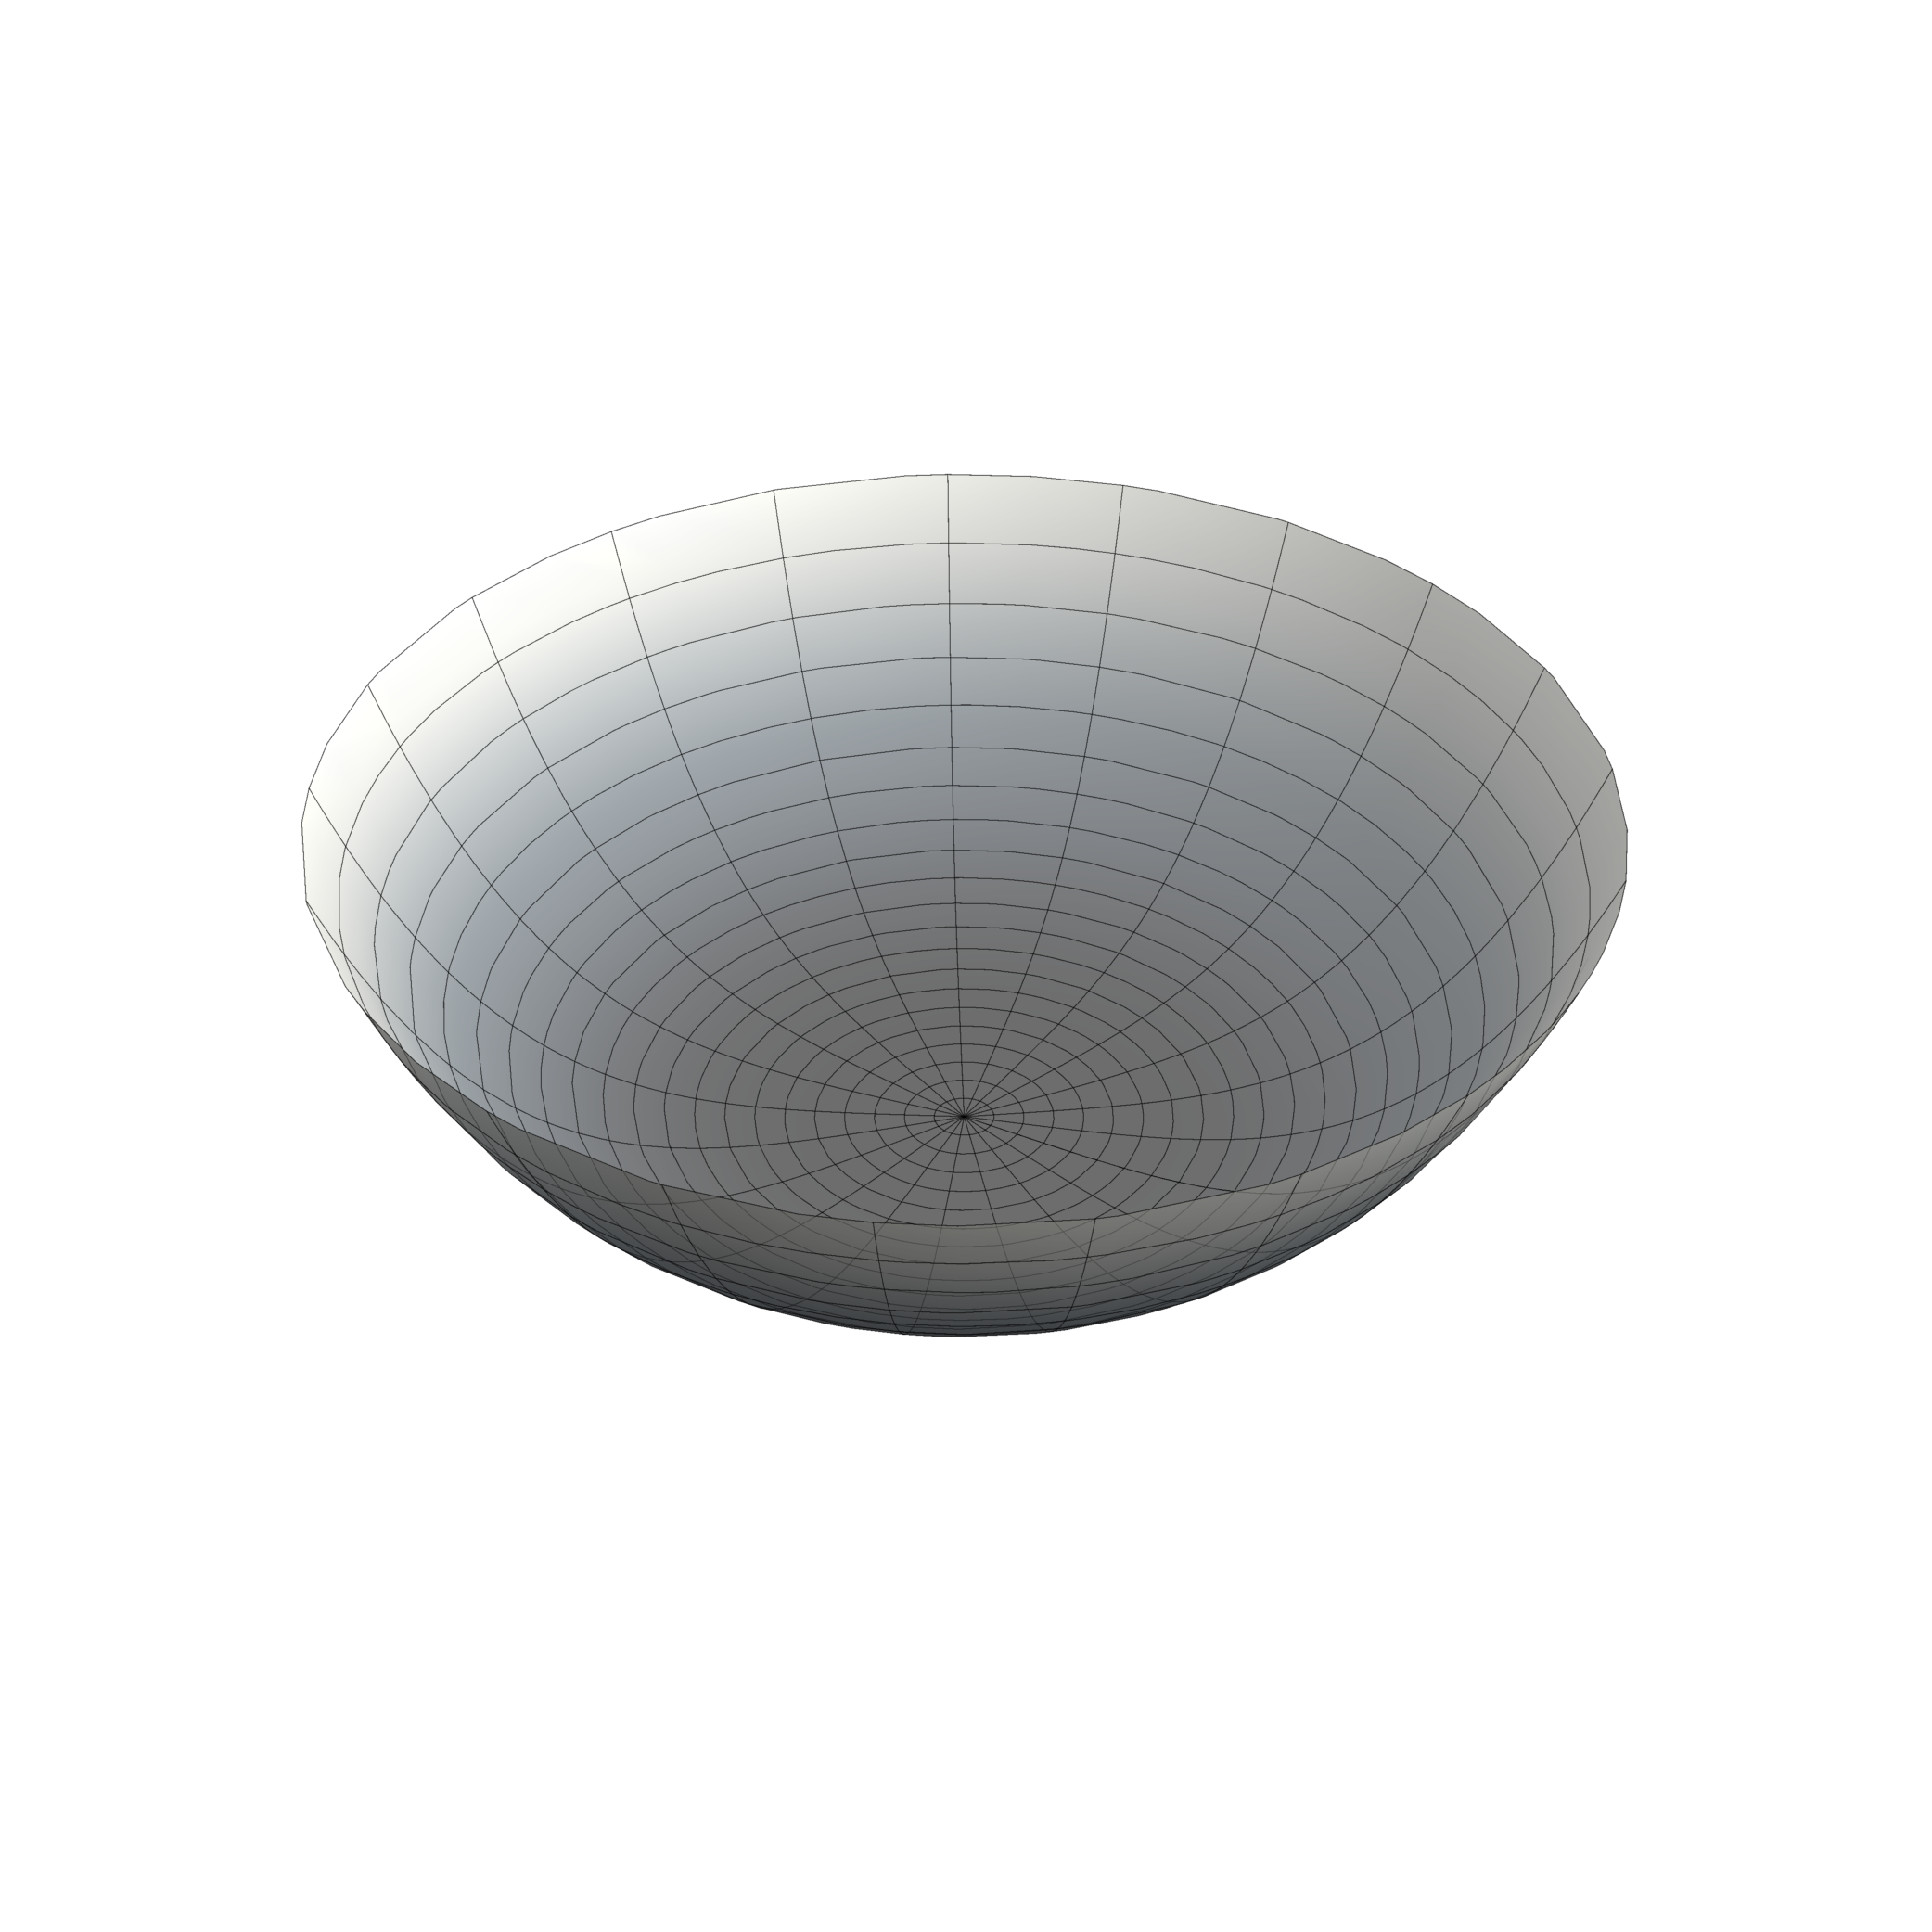
\includegraphics[width=0.75\linewidth]{Introduction/Non_Mexican_Hat.pdf}
\caption[A 2D illustration of the scalar potential, $V\left(\Phi\right)$, when $\mu^2 > 0$. The horizontal axes form the complex plane $\phi_{1}$ vs $\phi_{2}$, while the vertical axis is $V\left(\Phi\right)$.]{A 2D illustration of the scalar potential, $V\left(\Phi\right)$, when $\mu^2 > 0$. The horizontal axes form the complex plane $\phi_{1}$ vs $\phi_{2}$, while the vertical axis is $V\left(\Phi\right)$. Created with \cite{Mathematica10_1}.}
\label{fig:2Dsymmetry}
\end{center}
\end{figure}

\begin{figure}
\begin{center}
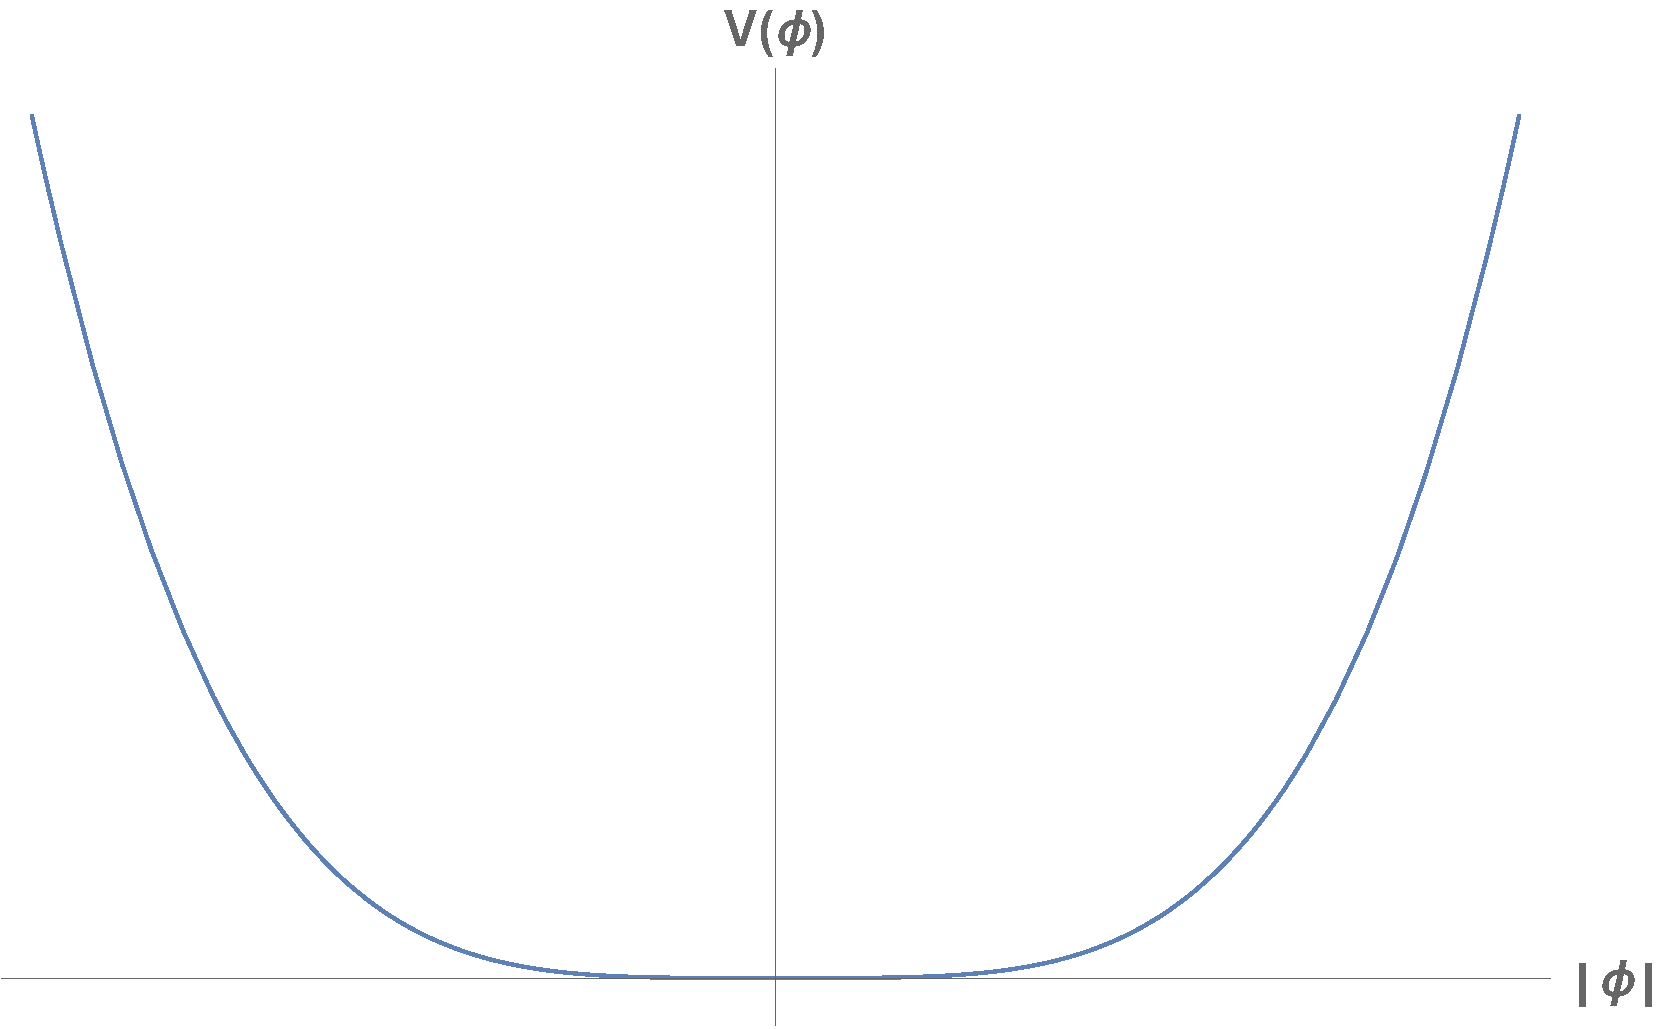
\includegraphics[width=0.75\linewidth]{Introduction/Non_Mexican_Hat_1D.pdf}
\caption[A 1D illustration of the scalar potential, $V\left(\Phi\right)$, when $\mu^2 > 0$.]{A 1D illustration of the scalar potential, $V\left(\Phi\right)$, when $\mu^2 > 0$. Created with \cite{Mathematica10_1}.}
\label{fig:1Dsymmetry}
\end{center}
\end{figure}

The more interesting case is when $\mu^2 < 0$. In this case the potential has a minimum that is not at $\Phi = 0$ but the minimum energy state will occur at what we call the \textit{vacuum expectation value} (VEV) given in equation \eqref{eq:VacExp}. This means that in the ground state, the scalar field will not go to zero but will have some amount of energy defined as $\frac{v}{\sqrt{2}}$ breaking the $\mathrm{U}(1)$ symmetry. Figures showing the natural two-dimensional potential and one-dimensional projection are seen in \ref{fig:2Dbroken} and \ref{fig:1Dbroken} respectively. 
\begin{equation}
\label{eq:VacExp}
\left<\Phi\right> = \sqrt{-\frac{\mu^2}{2\lambda}} \begin{pmatrix} 0 \\ 1 \end{pmatrix} \equiv \frac{1}{\sqrt{2}} \begin{pmatrix} 0 \\ v \end{pmatrix}
\end{equation}

\begin{figure}
\begin{center}
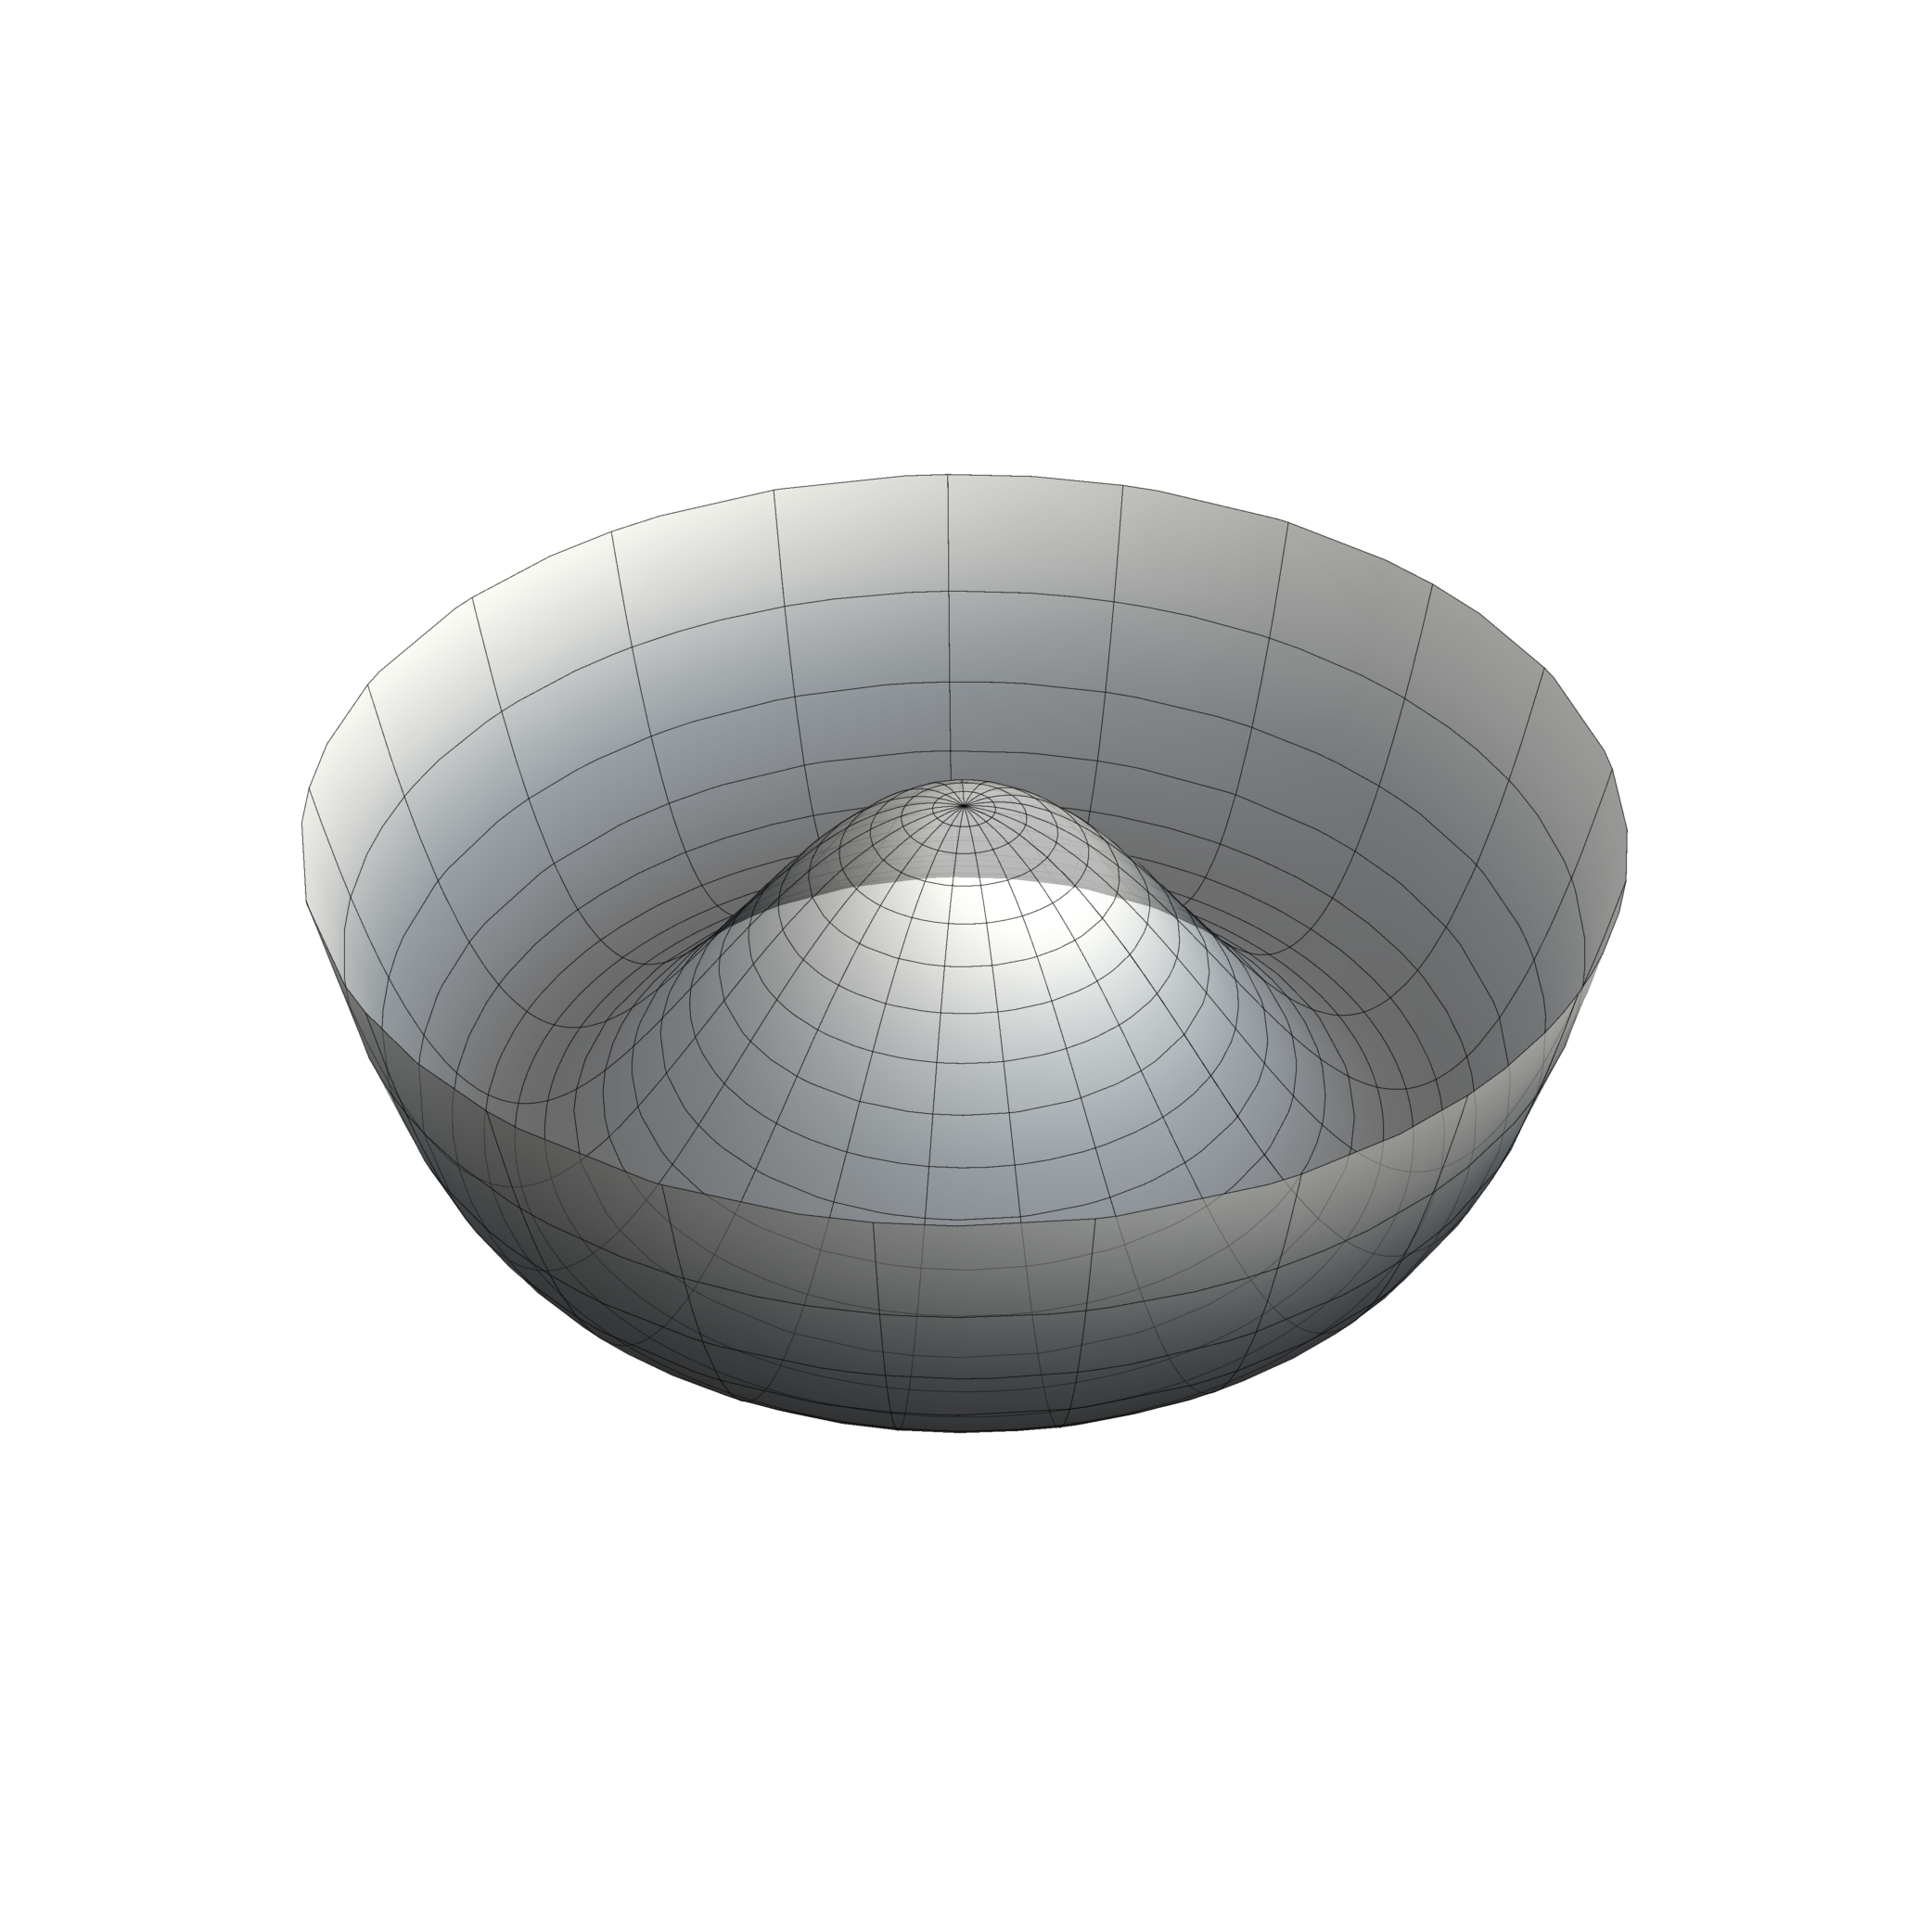
\includegraphics[width=0.75\linewidth]{Introduction/Mexican_Hat.pdf}
\caption[A 2D illustration of the scalar potential, $V\left(\Phi\right)$, when $\mu^2 < 0$. The horizontal axes form the complex plane $\phi_{1}$ vs $\phi_{2}$, while the vertical axis is $V\left(\Phi\right)$.]{A 2D illustration of the scalar potential, $V\left(\Phi\right)$, when $\mu^2 < 0$. The horizontal axes form the complex plane $\phi_{1}$ vs $\phi_{2}$, while the vertical axis is $V\left(\Phi\right)$. Created with \cite{Mathematica10_1}.}
\label{fig:2Dbroken}
\end{center}
\end{figure}

\begin{figure}
\begin{center}
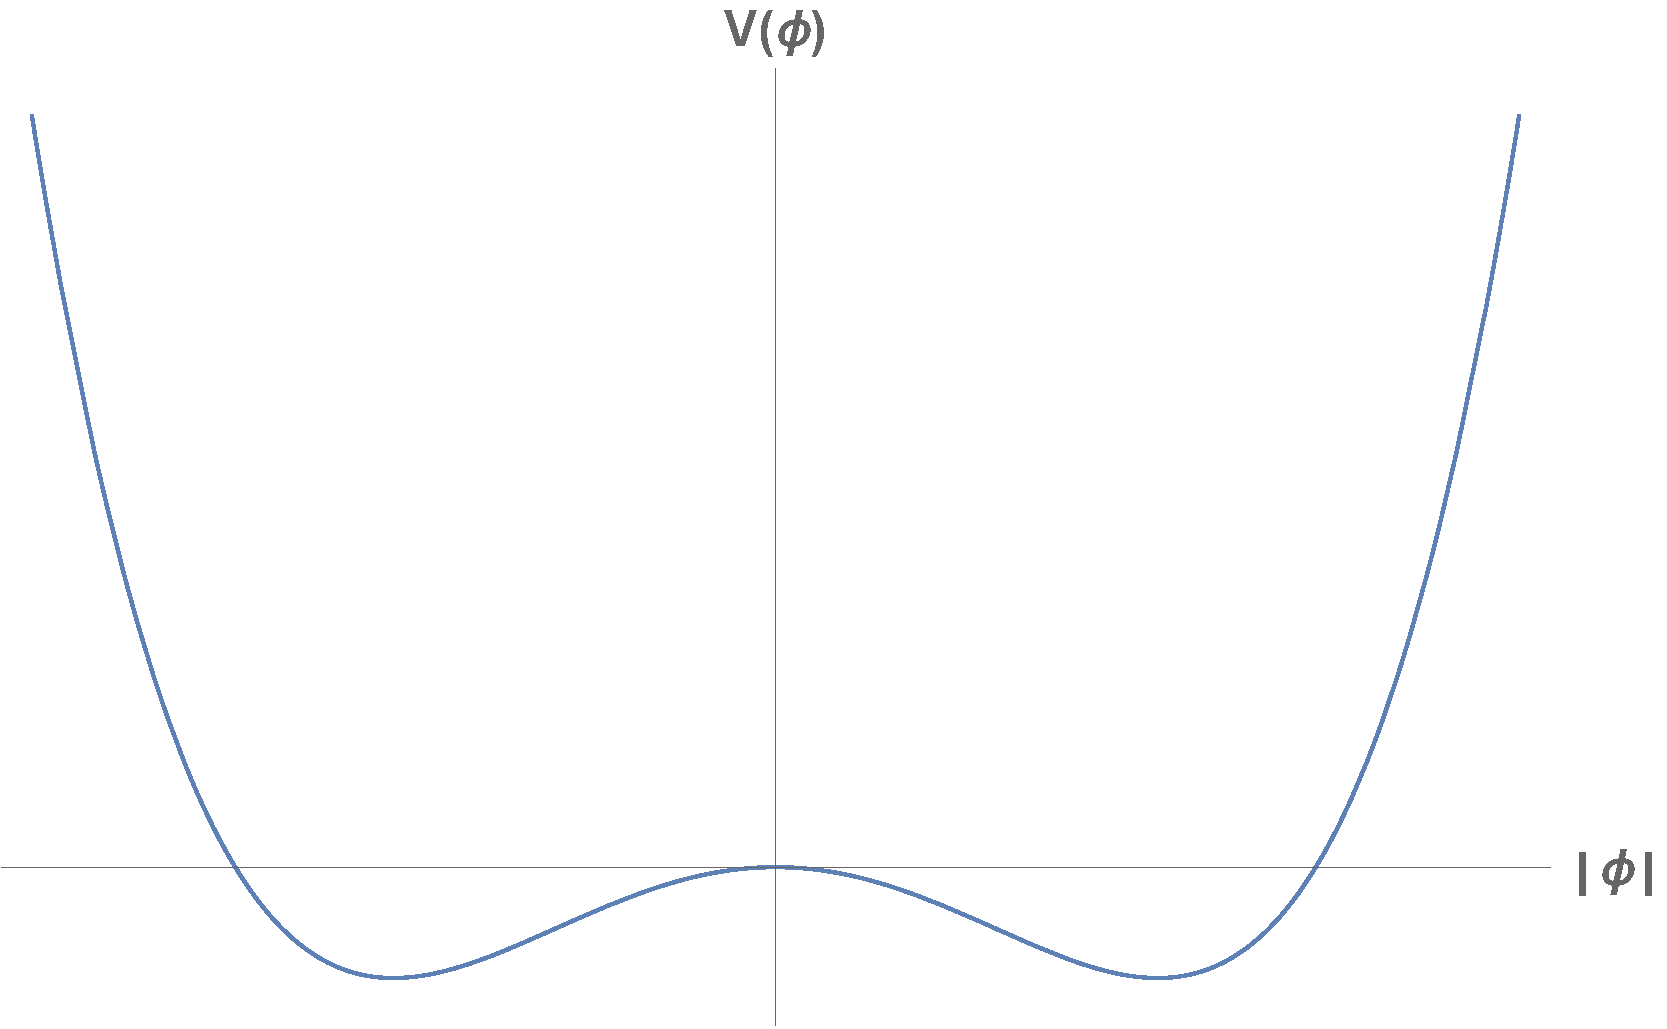
\includegraphics[width=0.75\linewidth]{Introduction/Mexican_Hat_1D.pdf}
\caption[A 1D illustration of the scalar potential, $V\left(\Phi\right)$, when $\mu^2 > 0$.]{A 1D illustration of the scalar potential, $V\left(\Phi\right)$, when $\mu^2 > 0$. Created with \cite{Mathematica10_1}.}
\label{fig:1Dbroken}
\end{center}
\end{figure}

The choice of the VEV contribution to the $\phi^{1}, \phi^{2}, \phi^{3} \text{ or } \phi^{4}$ component in $\mathrm{SU}(2)$ space is arbitrary but we have chosen the conventional notation here, giving the new doublet a hypercharge of $Y_{\Phi} = 1$ and a electromagnetic charge $Q_{EM} = \frac{\tau^{3} + Y}{2}$. This gives an electromagnetically neutral ground state, even though the field retains its VEV. So, by giving the scalar field a non-zero expectation value in the ground state we have broken the $\mathrm{SU}(2) \times \mathrm{U}(1)$ symmetry to give a local $\mathrm{U}(1)_{EM}$ symmetry of the electromagnetic force\footnote{As required by the Lorentz invariance of the electromagnetic force}.

We can see the difference between the masses of the original bosons by using the gauge invariance of the field to formulate our original scalar field $\Phi$ in terms of the VEV, $v$, and a remaining real scalar field, $h$, in equation \eqref{eq:vevPh}.

\begin{equation}
\label{eq:vevPh}
\Phi =  \frac{1}{\sqrt{2}} \begin{pmatrix} 0 \\ v + h \end{pmatrix}
\end{equation}

To see how these terms generate mass, it is convenient to perform a change of basis from $\tau^{1}, \tau^{2}, \tau^{3}$ to the $\tau^{+}, \tau^{-}, \tau^{3}$ representation given by equation \eqref{eq:PauliPM}. This change of basis also will change the $W^{1}_{\mu}, W^{2}_{\mu}, W^{3}_{\mu}$ to  $W^{+}_{\mu}, W^{-}_{\mu}, W^{3}_{\mu}$ given by equation \eqref{eq:Wpm}.
\begin{equation}
\label{eq:PauliPM}
\tau^{\pm}  =  \frac{1}{\sqrt{2}}\left(\tau^{1} \pm i \tau^{2}\right)
\end{equation}

\begin{equation}
\label{eq:Wpm}
W^{\pm}_{\mu}  =  \frac{1}{\sqrt{2}}\left(W_{\mu}^{1} \mp i W_{\mu}^{2}\right)
\end{equation}

Looking at the scalar kinetic term of equation \eqref{eq:EWsector}, $\left|\mathcal{D}_{\mu}\Phi\right|^{2}$, more explicitly we can write the boson terms in the form equation \eqref{eq:KEscalar}, dropping terms that represent the dynamics and interactions of the $h$ field.

\begin{equation}
\label{eq:KEscalar} 
\frac{v^2}{4}\left(g_{2}W_{\mu}^{3} - g_{1}B_{\mu}\right)^2 + \frac{g_{2}^{2}v^{2}}{2}W_{\mu}^{+}W^{\mu -}
\end{equation}

After another change of basis, we can recast the first term in equation \eqref{eq:KEscalar} as the physical gauge fields we observe in nature. In equations \eqref{eq:AandZ} and \eqref{eq:masses}, we see the $Z$ and $\gamma$ fields we are looking for and the masses of the bosons respectively. 

\begin{eqnarray}
\label{eq:AandZ}
Z_{\mu}  &=&  \frac{g_{2}W^{3}_{\mu} - g_{1}B_{\mu}}{\sqrt{g_{1}^{2}+g_{2}^{2}}} \nonumber \\
A_{\mu}  &=&  \frac{g_{2}W^{3}_{\mu} + g_{1}B_{\mu}}{\sqrt{g_{1}^{2}+g_{2}^{2}}}
\end{eqnarray}

\begin{eqnarray}
\label{eq:masses}
m_{W} & = & \frac{v}{\sqrt{2}}g_{2} \nonumber \\
m_{Z} & = & \frac{v}{\sqrt{2}}\sqrt{g_{2}^{2} + g_{1}^{2}} \\
m_{\gamma} & = & 0 \nonumber 
\end{eqnarray}

Thus we have broken the electroweak symmetry, giving the $W^{\pm}$ and $Z$ bosons mass while keeping the $\gamma$ massless. This provides a theory that predicts a new field, $h$, called the \textit{Higgs field}, and allows us to describe the behavior of the weak and electromagnetic forces to fantastic accuracy. 

To investigate the ramifications of this new field, we can formulate the $h$ field as small permutations about the VEV. This gives a potential of the form $\phi\left(x\right) = v + \frac{1}{\sqrt{2}}\left(\chi\left(x\right) + i\psi\left(x\right)\right)$. These permutations are illustrated in figure \ref{fig:Oscillate}. From the figure it is clear that a small displacement in $\psi$ does not cost energy, while oscilations in $\chi$ do cost energy. Thus $\chi$ corresponds to a new massive boson is called the \textit{Higgs Boson} in common literature. Everything about this new boson can be predicted from the SM, except the two parameters, $\mu^{2}$ and $\lambda$, or equivalently the VEV given in equation \eqref{eq:VeV} and the mass of the Higgs Boson in equation \eqref{eq:Hmass}.

\begin{figure}
\begin{center}
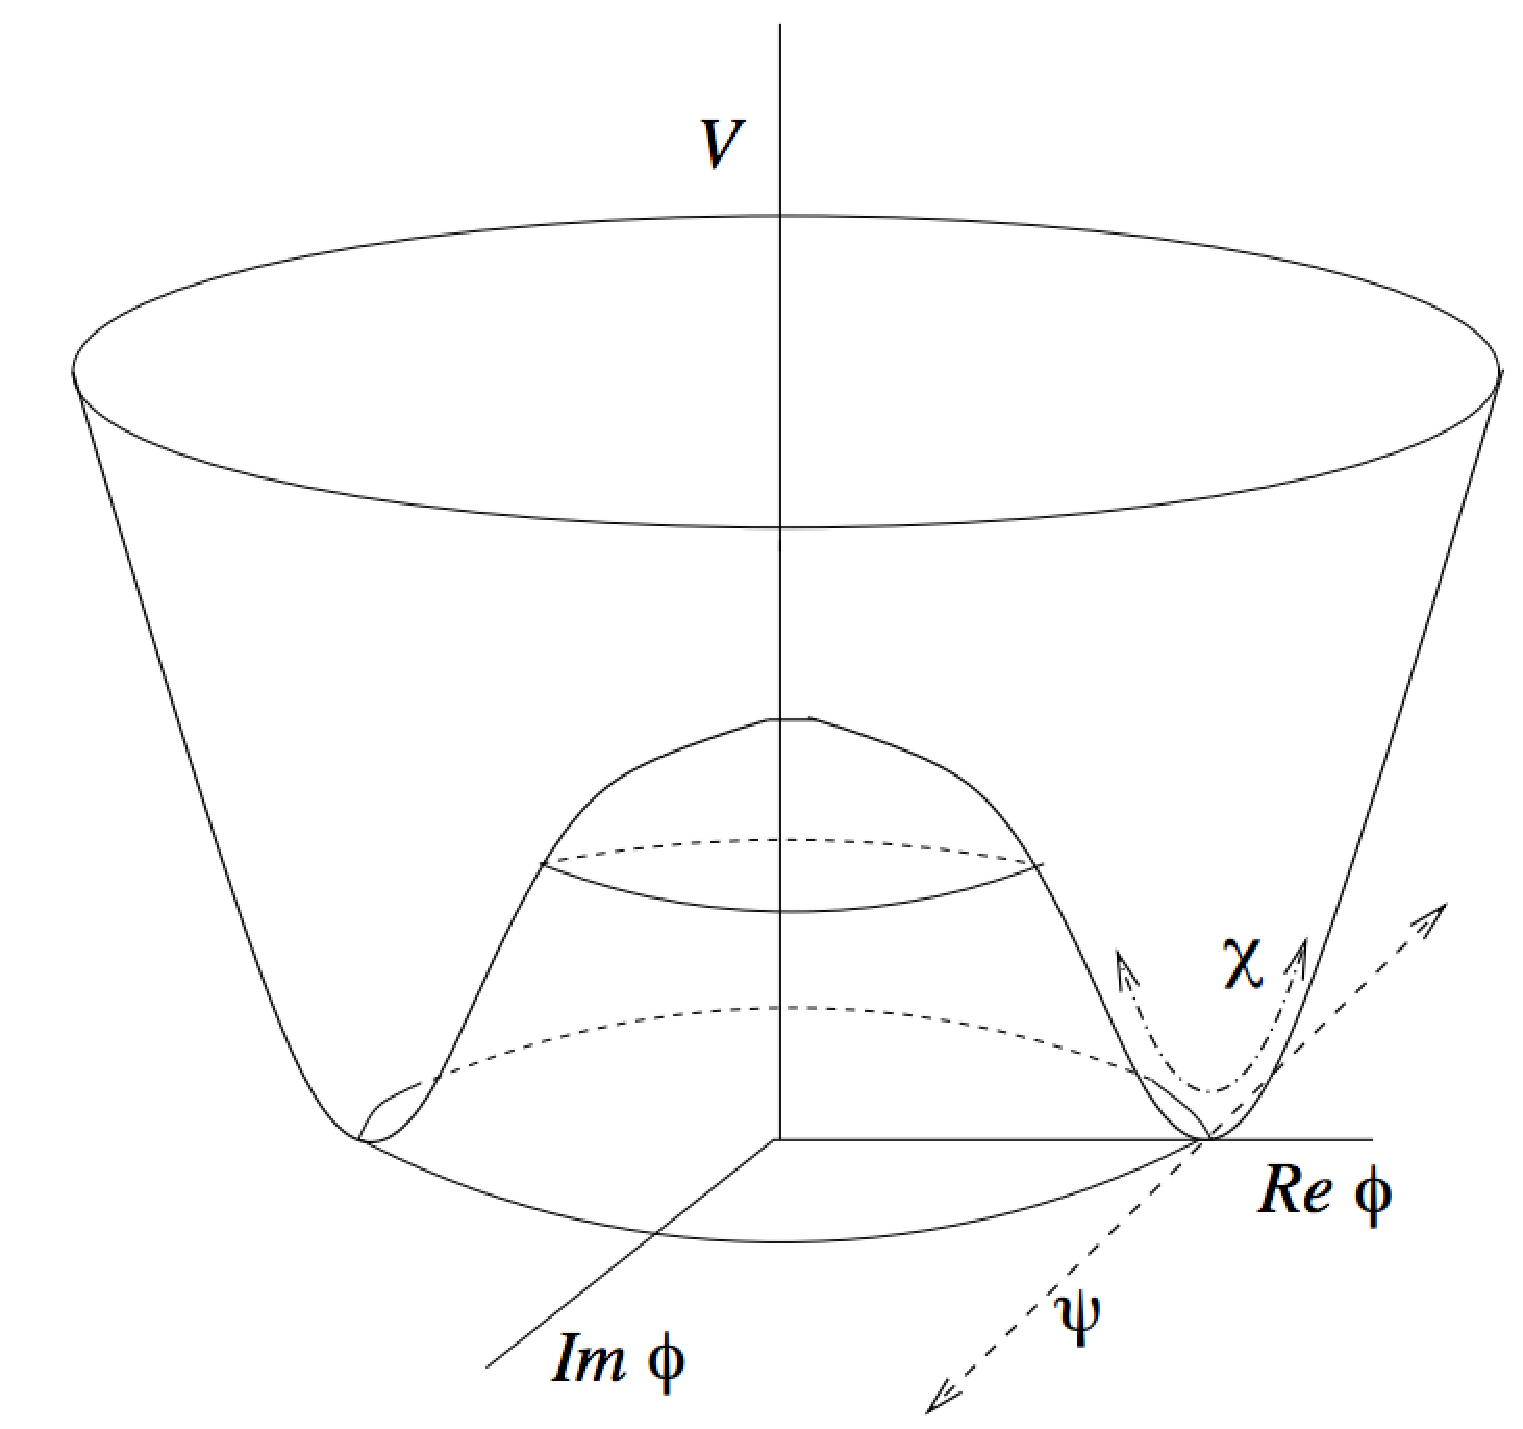
\includegraphics[width=0.75\linewidth]{Introduction/Oscillations_VEV.pdf}
\caption[A 2D illustration of oscillations in the the scalar potential, $V\left(\Phi\right)$, parameterized by $\chi$ and $\psi$.]{A 2D illustration of oscillations in the the scalar potential, $V\left(\Phi\right)$, parameterized by $\chi$ and $\psi$ \cite{Maggiore11.2:2005}.}
\label{fig:Oscillate}
\end{center}
\end{figure}

\begin{equation}
\label{eq:VeV}
v^{2} = -\frac{\mu^2}{2\lambda}
\end{equation}

\begin{equation}
\label{eq:Hmass}
m_{h}^{2} = 2v^{2}\lambda
\end{equation}

\subsubsection{Implications of the Higgs field: Fermion Masses}
\label{sec:FermionMasses}

When we first started our discussion of Fermions we simply wrote the mass of a fermion as $-m\bar{\psi}\psi$ in equation \eqref{eq:EMlagrangian}. However, this term would explicitly break the electroweak gauge invariance we have just spent so much time constructing. It turns out that the new scalar field $h$ could also be responsible for the fermion masses in addition to the $W^{\pm}$ and $Z$ masses. The term can be created by considering a Yukawa coupling between the scalar field and a fermion field. For the down quark this term follows equations \eqref{eq:Yd}\footnote{In these equations h.c. stands for the hermitian conjugate term.}.

\begin{eqnarray}
\label{eq:Yd}
\mathscr{L}_{\mathrm{d-mass}} &=& -\lambda_{d}\bar{Q_{L}}\Phi d_{R} + h.c. \nonumber \\
 &=& \frac{-\lambda_{d}}{\sqrt{2}}\begin{pmatrix}\bar{u_{L}}& \bar{d_{L}}\end{pmatrix}\begin{pmatrix} 0 \\ v + h \end{pmatrix} d_{R} + h.c. \\
  &=& \frac{-\lambda_{d}v}{\sqrt{2}}\bar{d_{L}}d_{R} + h.c. \nonumber
\end{eqnarray}

Where the final equality comes from focusing on the terms that remain in the ground state of the scalar potential. From here its easy to see that the mass of the down quarks can be obtained from the vacuum expectation value of the scalar field and the down coupling to the Higgs field, $\lambda_{d}$.

\begin{eqnarray}
\label{eq:Md}
m_{d} = \frac{\lambda_{d}v}{\sqrt{2}} \nonumber
\end{eqnarray}

The masses of the other fermions follow from equations similar to \eqref{eq:Yd} where the Higgs field, $h$, interacts with all the fermions. This will be the key to generating Higgs bosons at the LHC, particularly Higgs couplings to top quarks.

It seems that the Higgs Mechanism and the Higgs boson solve many of the issues that the SM has with describing the world we observe. However, there are many other unexplained phenomena in the universe and detailed study of the Higgs mechanism could lead unearth the origin of these discrepancies. The next subsection is an outline some of these discrepancies that will be discussed in this document.

\section{Limitations of the SM: Higgs boson as a tool}
\label{sec:Limitations}

The SM has been one of the most successful scientific theories ever proposed. The predictive power of the model is unparalleled, yet some questions remain. The first limitation we will discuss in this section will be the matter-antimatter asymmetry seen in the universe around us. Secondly, a discussion of the SM's inability to accurately describe gravity is presented. Finally, generalizations of the SM are discussed. These models that could generate the dark matter seen in astronomical measurements, solve the hierarchy problem, or explain more about fermions. The Higgs field could offer keys to understanding all of these issues and the tests presented in this document are intended to address these questions.

\subsection{$CP$-volation: The Matter-Antimatter Asymmetry}
\label{sec:CPviolation}

Outside of specific particle physics experiments, the universe we live in is dominated by matter. It seems that only a very small fraction of antimatter exists in the universe. However, within specific tests of SM no process is observed to generate this large of a discrepancy between matter and antimatter. Under the assumption that matter and antimatter started in equal amounts, after the Big Bang, matter and antimatter should still exits in relatively equal densities and amounts. The SM does not predict, nor has any experiment seen, a process that could generate enough $CP$-violation to create a universe that is so overwhelmingly dominated by matter.

So far we have only eluded to $CP$ transformations when introducing the antiparticles that exist in the SM. In the most basic terms this is the combination of two discrete symmetries \textit{charge conjugation} and \textit{parity symmetry} (spatial inversion). The parity operation, $P$, is the spatial inversion through the origin. We saw the projections of a fermion onto the eigenstates of this operation at the end of section \ref{sec:SU2}. If $\psi\left(x\right)$ describes a fermion field at point $x$, then $P\psi\left(x\right) \to \psi\left(-x\right)$. This transformation will take $x \to -x$ and the momentum $p \to -p$ but leave the inherent spin and other quantum numbers unchanged. The charge conjugation operation, $C$, is the transformation of a particle to its antiparticle or vice versa. We used this transformation extensively in \ref{sec:TheSM} but never wrote out the transformations explicitly. As an example, given an electron, $e^{-}$, then $Ce^{-} \to e^{+}$. This transformation will reverse the sign of all quantum numbers associated with the particle (inherent spin, weak isospin, charge, hypercharge, etc...). Particles that are their own antiparticle ($\pi^0$ meson, $\nu$'s, ...) remain unchanged under this operator (aside from a possible factor of -1).

Not all interactions allowed by the standard model will preserve these symmetries. The most explicit example is the weak interaction. Given that the weak force only interacts with left-handed particles, it is maximally parity violating\footnote{Imagine a stationary pseudoscalar $\pi^{+}$ decaying into back-to-back $\mu^{+}$ and $\nu_{\mu}$ states via the weak interaction. Perform the parity operation on the initial and final states. The result requires a right-handed neutrino, which are unobserved.}. However, in most cases $CP$ together is a symmetry of the interactions. The notable exceptions to this are the decays of B mesons and Kaons \cite{Agashe:2014kda}. These decays highlight the necessity for a $CP$-violating component in the SM described by the Cabibbo-Kobayashi-Moskawa Model \cite{Kobayashi:1973fv}. The specifics of this model are beyond the scope of this document. However, the observed magnitudes of the terms in the CKM model cannot account for the large discrepancy that we observe in the universe.

One proposed solution to this asymmetry is the presence of more than one Higgs field, resulting in multiple Higgs bosons. The number of fields and bosons predicted varies depending to the model and any observed boson could have varied spin $(J)$, charge $(C)$, and parity $(P)$ transformation properties. It could be charged, neutral, pure scalar, pure pseudoscalar, vector, pseudovector or a mixed vector-pseudovector state. In this document we outline tests proposed and performed to test the $J^{CP}$ nature of a boson to see if a Higgs boson can offer any insights into the nature of the matter-antimatter asymmetry.

\subsection{The Graviton: An Unexplained Force}
\label{sec:Graviton}

Gravity would be the weakest of all the forces we know of but it is not yet included in the SM. There are many possible theories of gravity at small scales and its corresponding boson, the \textit{graviton}. In Table \ref{tab:Forces} you can find a summary of the different forces and their relative strengths and interaction ranges, including gravity. Since gravity is so intimately connected with the mass of an object in relativistic mechanics it is expected to have similar couplings to the SM particles as the Higgs boson, but to match general relativity most theories claim that it must be a spin-2 particle. Generally, most theories predict that a graviton would be a massless particle to have an infinite interaction range. There is always the possibility of new physics spoiling our expectations so a detailed study of any new scalar particle found should be performed to determine if the spin is zero (as predicted by Higgs boson) or two (as predicted by a Beyond SM graviton).

In this analysis, we study a few possibilities for a graviton-like particle. This is discussed in more detail in section \ref{sec:Spin2_Pheno}, but generally we consider a Kaluza-Klein theories where a closed fifth dimension could give rise to a massive spin two graviton \cite{Klein:1926fj}. Exact definitions of the models tested, and references motivating them can be found in section \ref{sec:Spin2_Pheno}.


\subsection{Beyond the SM: The Dark Matter, Hierarchy \& Fermion Problems}
\label{sec:BSM}

It has not been explicitly expressed in our discussion of SM phenomena but everything that we understand about the universe is really only valid at masses up to a certain sclae $\left(\sim m_{W/Z}\right)$. Using current models of the early universe, at early times we know that the energies are many orders of magnitude larger than what our SM theory can describe \cite{Weinberg:1977ji}. Many extensions of the SM to these high energies have been proposed and generally we will call them Beyond SM (BSM) theories in this document. These theories predict varied and wide ranging possibilities for new particles and physics and could be tested by examining a Higgs boson. Some BSM theories predict particles that could exist in relative obscurity on Earth but could be the \textit{dark matter} observed in astronomical experiments \cite{Trimble:1987ee}. 

Currently there is no explanation for why gravity is so much weaker, table \ref{tab:Forces}, than the other forces. The SM requires a very specific values in order to explain this difference without theoretical motivation. This is called the \textit{hierarchy problem} of the SM.  BSM theories offer natural solutions to this problem sometimes simultaneously with explanations for the dark matter abundance. Other issues that can be explained through BSM theories include the number of fermion generations and their masses. In principle, there is no preference for only three generations of fermions and not motivation for the specific masses of these particles. 

Generally, BSM theories can come in almost any type imaginable. If these new particles interact with the scalar $\Phi$ field, then they could be seen as a deviation from the expected couplings (interactions) with SM particles. These deviations could take many forms, but those tested in this document include: Unusual production mechanisms, unexpected spin-parity behavior, and enhanced non-resonant production.
